\documentclass[a4paper, 12pt]{article}

% čeština & angličtina
\usepackage[utf8]{inputenc}
\usepackage[version=4]{mhchem}
\usepackage[english,czech]{babel}
\usepackage{bakalarska_prace}
\usepackage{url}

%%

% citace
\usepackage[nottoc]{tocbibind}

% kód
\usepackage{listings}
\usepackage{minted}
\definecolor{codegreen}{rgb}{0,0.5,0}
\definecolor{codegray}{rgb}{0.5,0.5,0.5}
\definecolor{darkcyan}{rgb}{0.0, 0.55, 0.55}
\definecolor{backcolour}{rgb}{0.98,0.98,0.98}
\definecolor{royalblue(traditional)}{rgb}{0.0, 0.14, 0.4}
\definecolor{darklavender}{rgb}{0.45, 0.31, 0.59}

%Code listing style named "mystyle"
\lstdefinestyle{mystyle}{
  backgroundcolor=\color{backcolour},   commentstyle=\color{codegreen},
  emph={self},
  emphstyle={\color{darklavender}},
  keywordstyle=\color{royalblue(traditional)},
  numberstyle=\tiny\color{codegray},
  stringstyle=\color{darkcyan},
  basicstyle=\footnotesize\ttfamily\color{black},
  breakatwhitespace=false,         
  breaklines=true,                 
  captionpos=b,                    
  keepspaces=true,                 
  numbers=left,                    
  numbersep=5pt,                  
  showspaces=false,                
  showstringspaces=false,
  showtabs=false,                  
  tabsize=2
}

%"mystyle" code listing set
\lstset{style=mystyle}

%%

% grafika
\usepackage{graphicx}
\usepackage{wrapfig}
\usepackage{caption}
\usepackage{subcaption}
\usepackage{color, soul}
\usepackage[usenames,dvipsnames]{xcolor}
\usepackage[most]{tcolorbox}
\newtcolorbox{highlighted}{colback=yellow!40,coltext=black,breakable}

%\usepackage{tikz}
\newcommand*{\Icon}{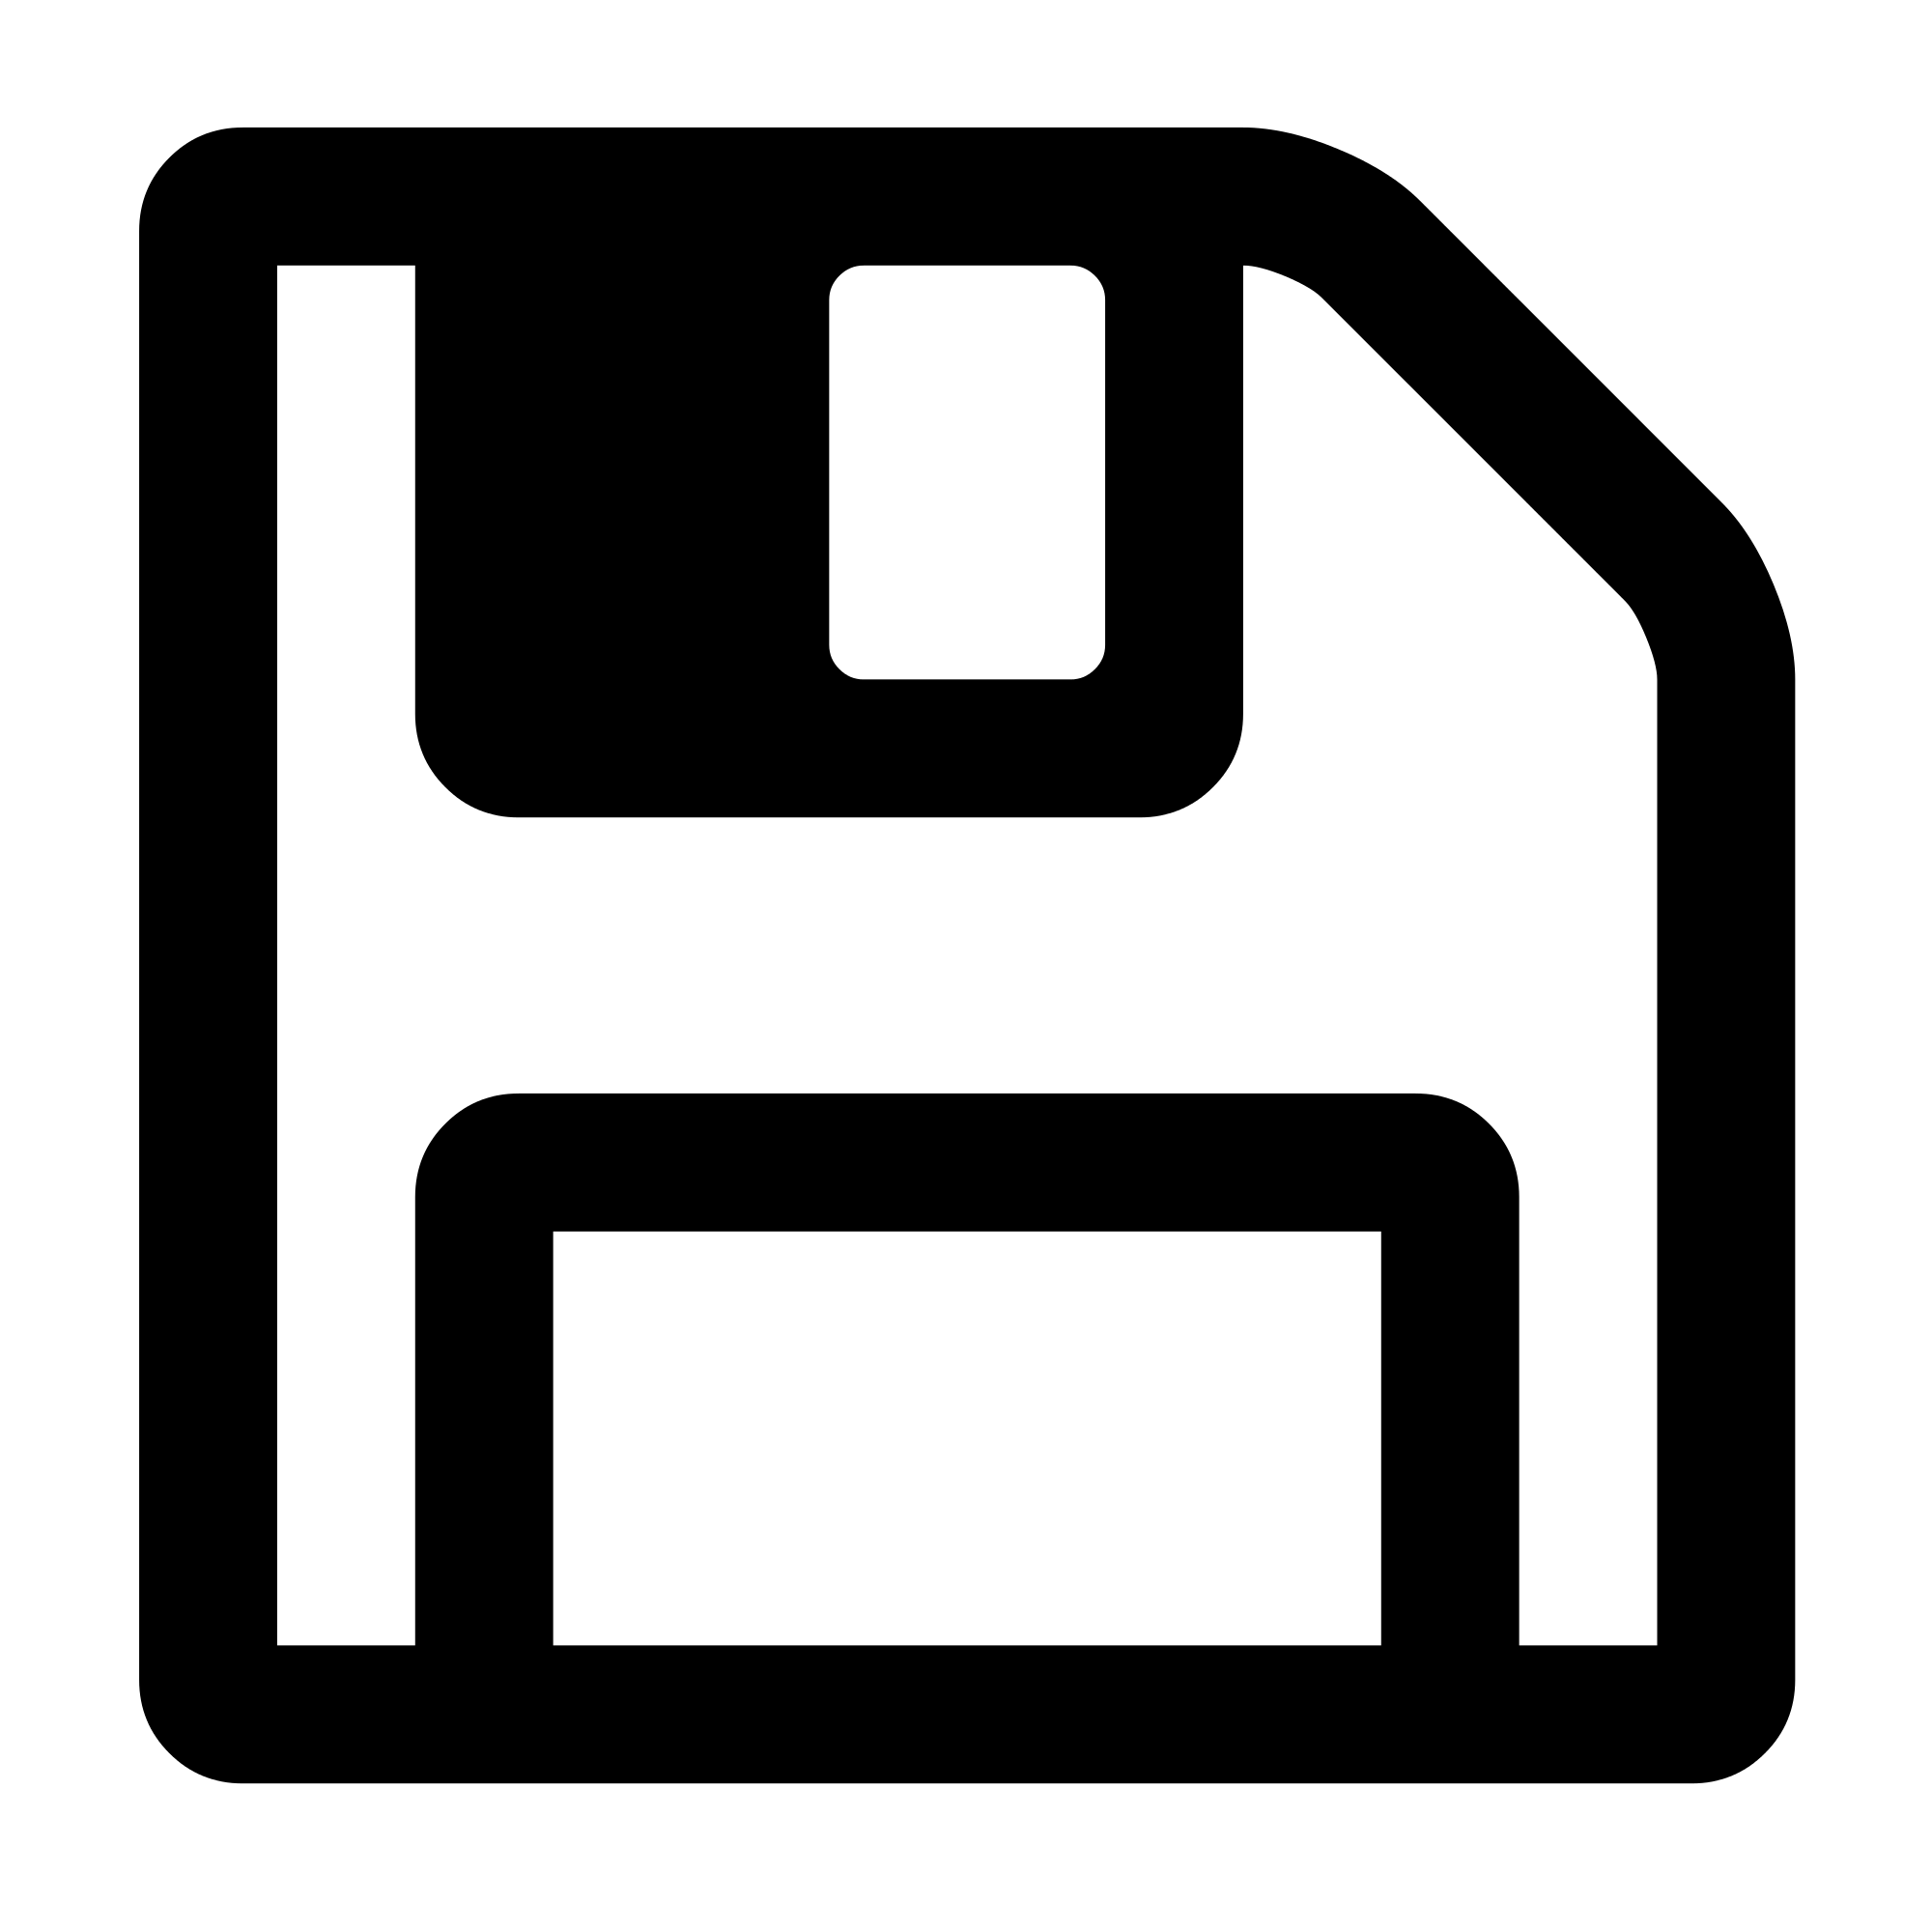
\includegraphics[width=0.5cm, height=0.5cm]{icon.PNG}}%


% okraje (v případě potřeby):\usepackage[showframe]{geometry}
%%

% poznámky
\usepackage[colorinlistoftodos]{todonotes}
\newcommand\todoin[2][]{\todo[inline, caption={2do},#1]{\begin{minipage}{\textwidth-4pt}#2\end{minipage}}}
\definecolor{lavender}{rgb}{0.96, 0.73, 1.0}
\definecolor{cdorange}{rgb}{0.93, 0.53, 0.18}
%
\newcommand{\cR}{\color{red}}
\newcommand{\misRef}{{\cR[REF]\,}}
\newcommand{\cB}{\color{blue}}
%%

% matika
\usepackage{amsmath} 
%%
\usepackage{pdfpages} 

\begin{document}
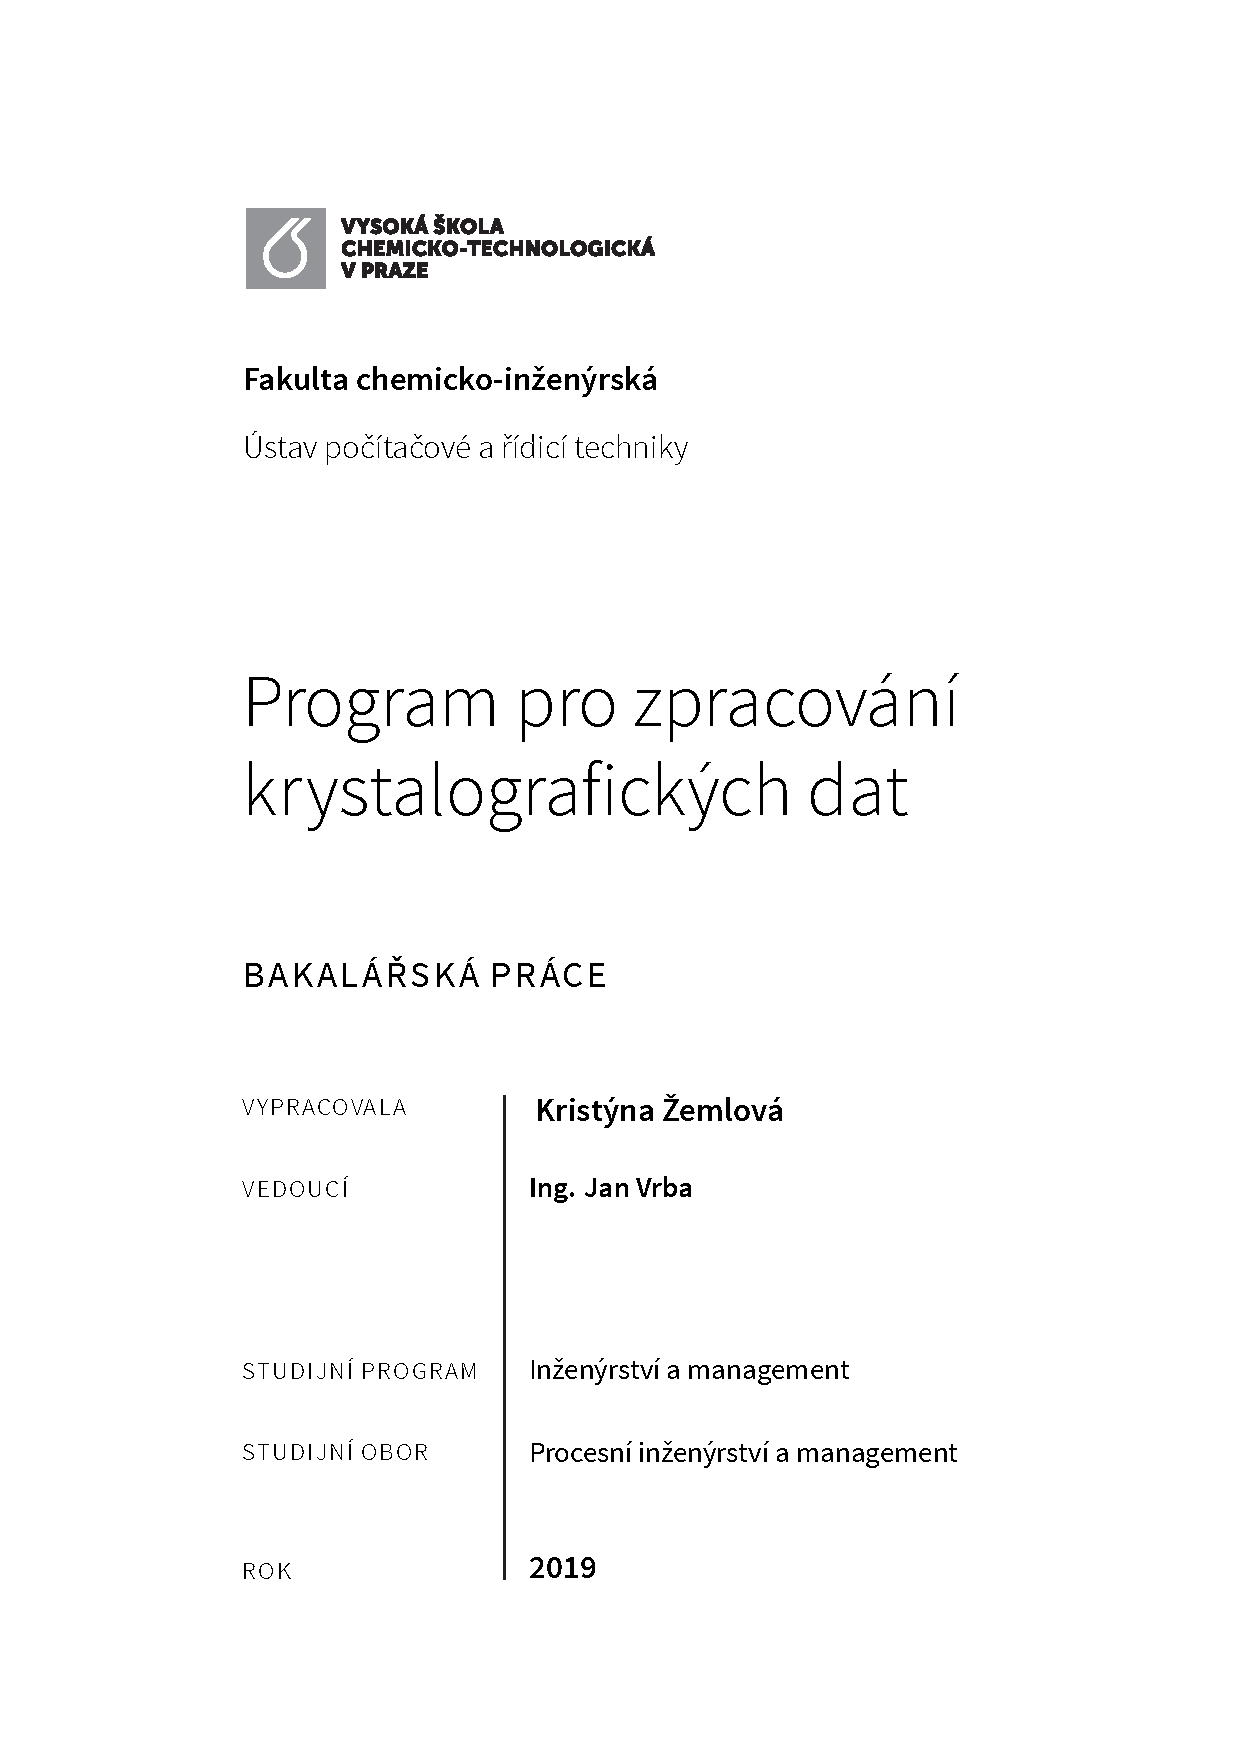
\includepdf{vstupni_listy.pdf}
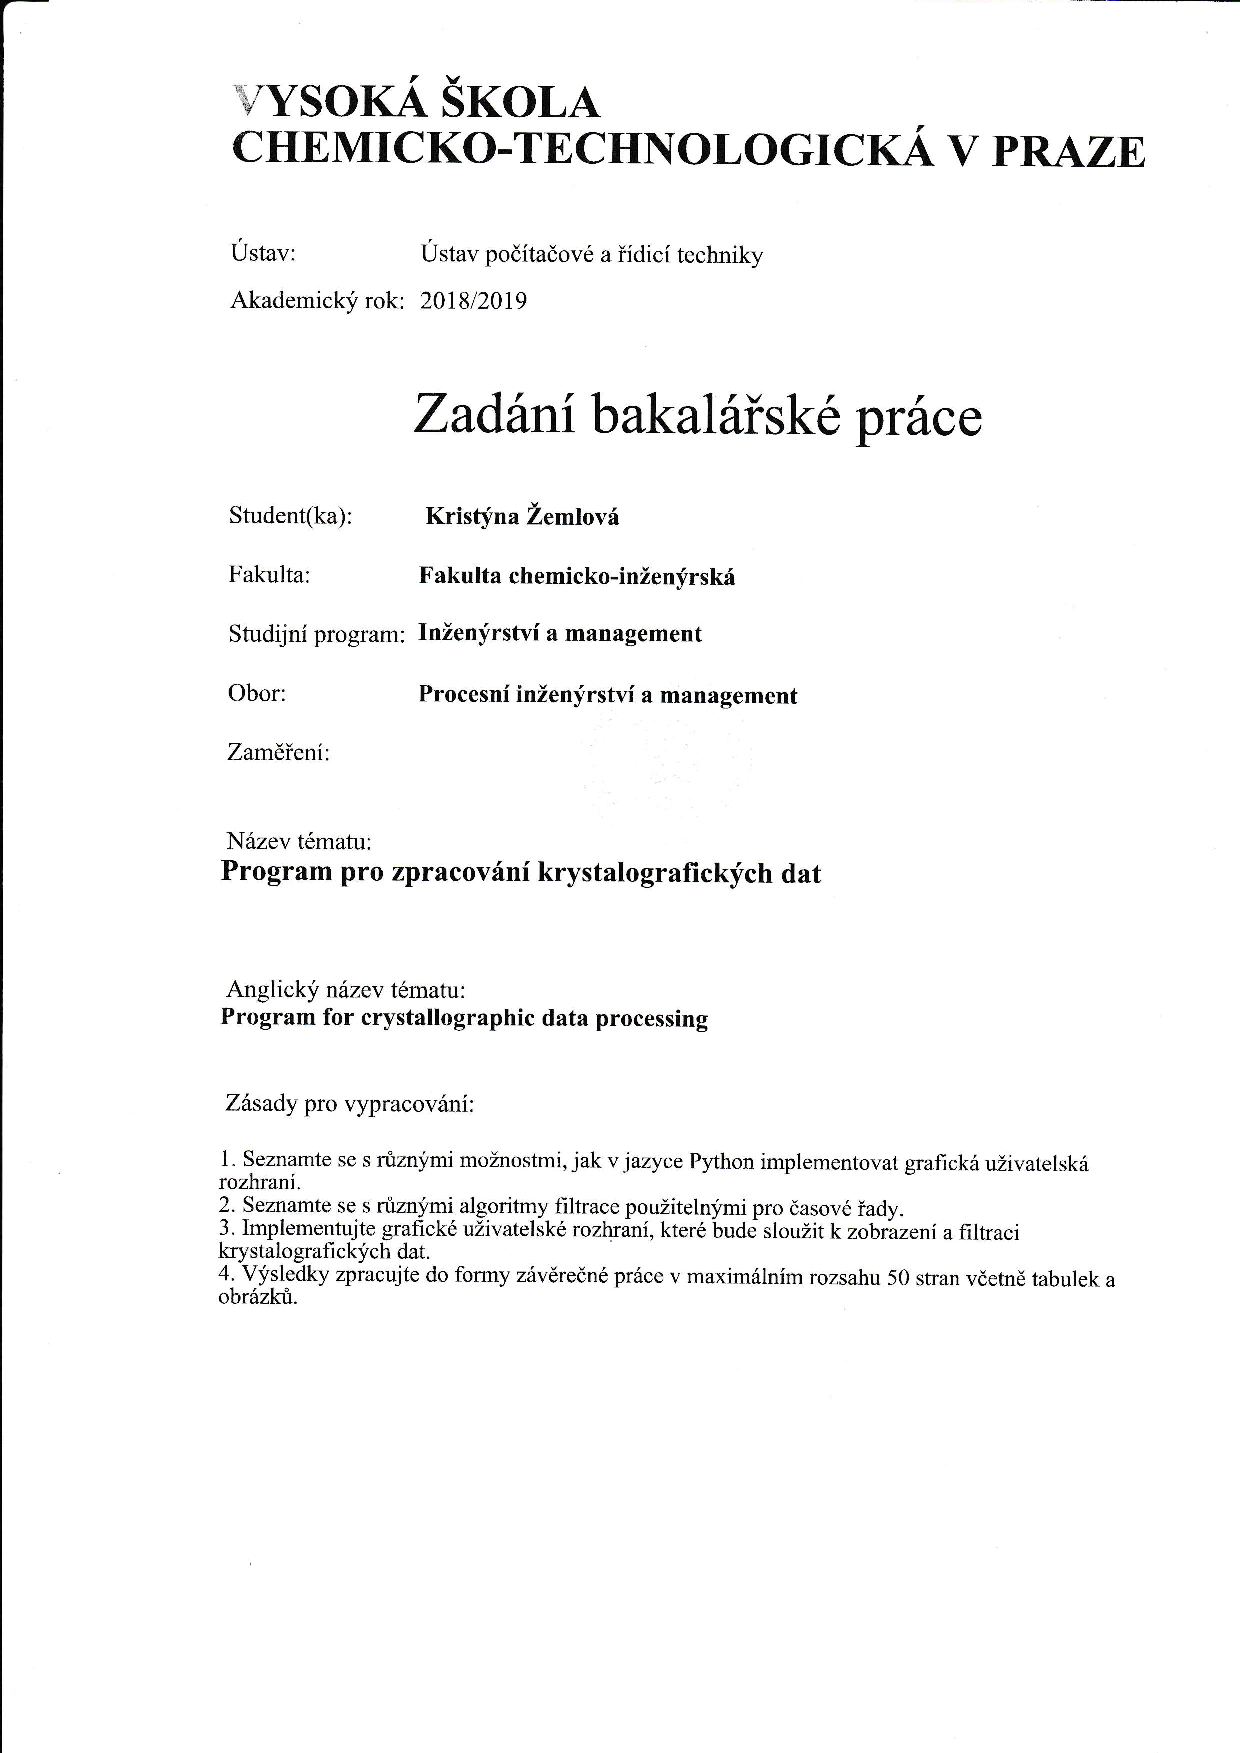
\includepdf{zadani_1.pdf}
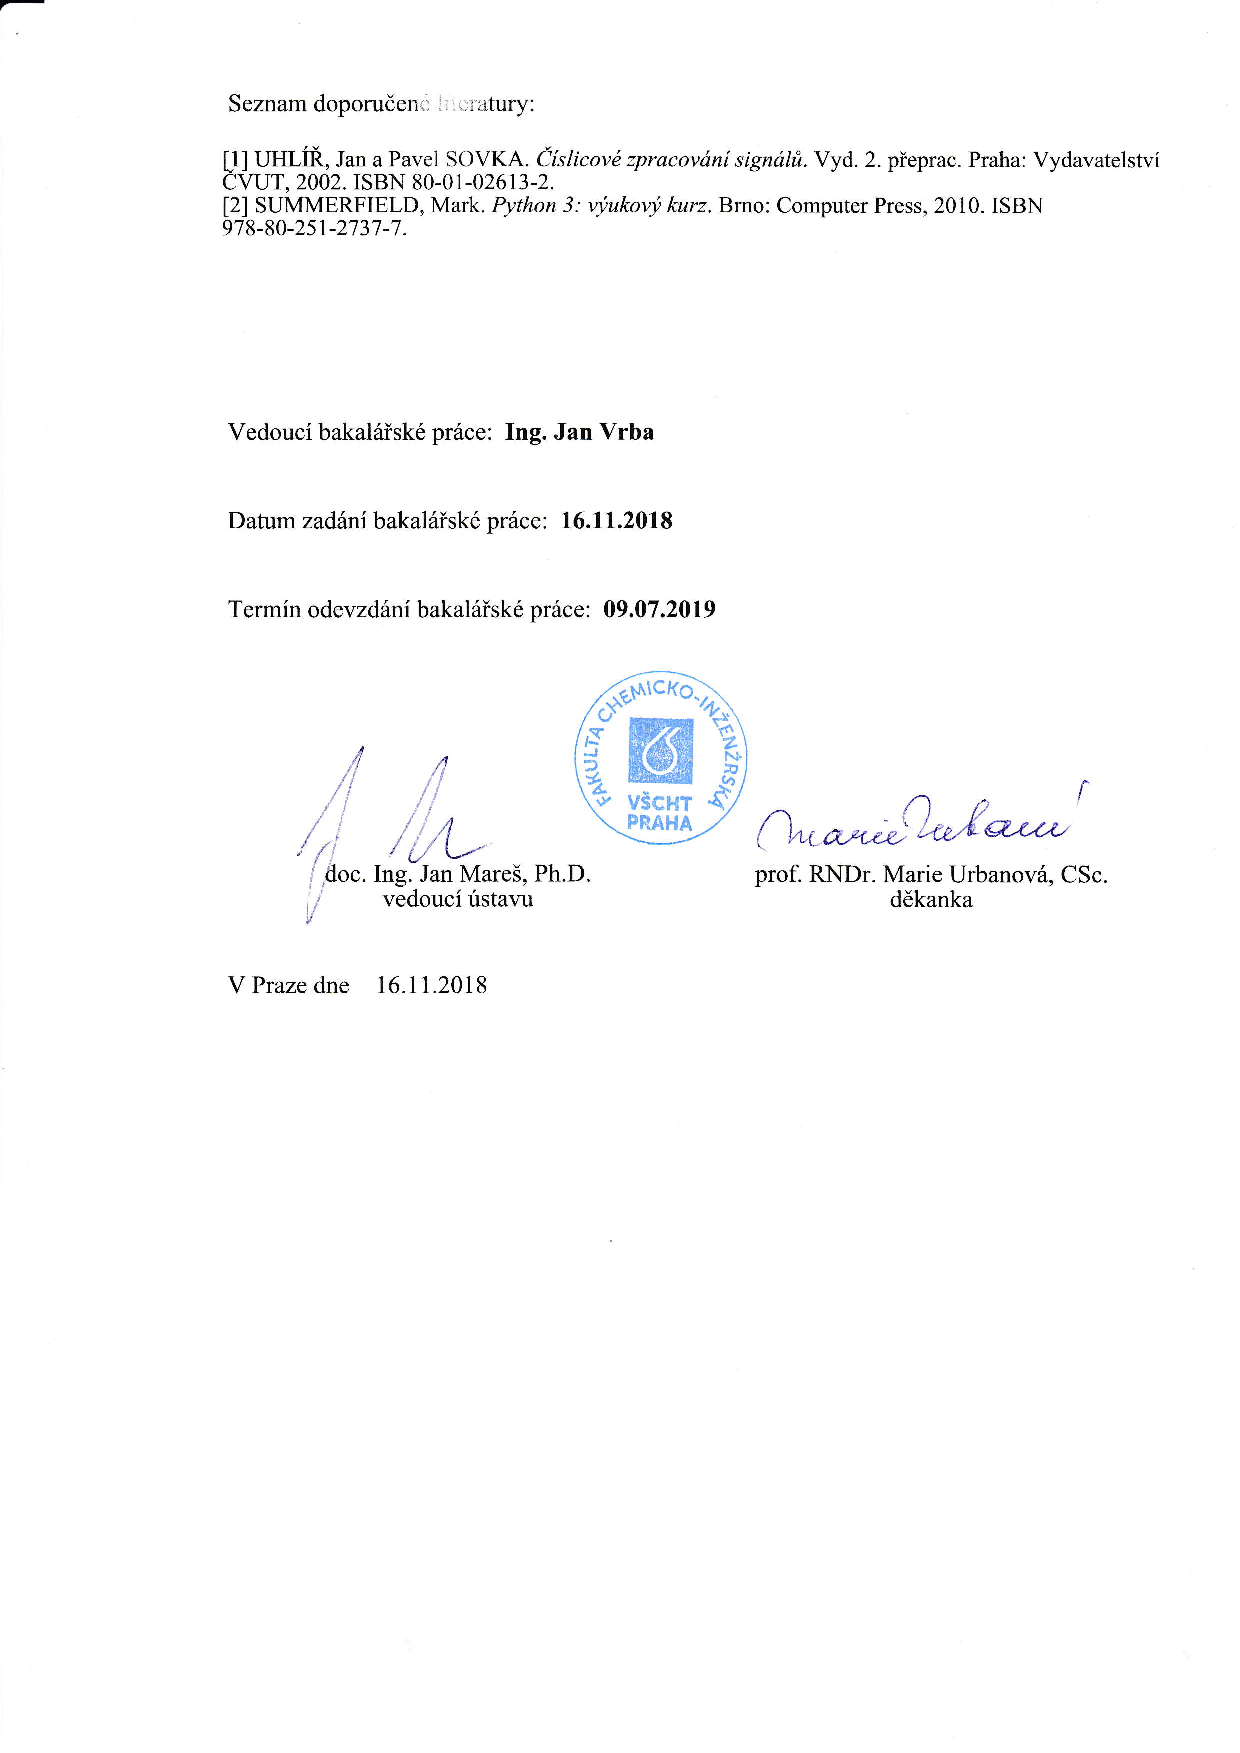
\includepdf{zadani_2.pdf}

% souhrn
% (CZ)
\begin{abstract}
Při reaktivní sintraci dochází působením tlaku a tepla ke spékání práškových kovů za vzniku jejich sloučenin. Pro zkoumání mechanismu a kinetiky tohoto děje se využívá snímání reakční směsi pomocí \textit{in situ} rentgenové difrakce. Z takto získaných dat lze zpětně vizuálním posouzením přibližně identifikovat  moment vzniku jednotlivých intermetalických sloučenin. Cílem této práce bylo vytvořit program s uživatelským rozhraním umožňující efektivnější analýzu krystalografických dat s důrazem na přesnost identifikace vznikajících fází. Vzniklý program je vybaven nástroji pro načítání dat ze souborů, jejich vizualizaci a zpracování signálu. Program rovněž umožňuje zpracovaná data zpětně exportovat do souborů. K tvorbě programu byl využit programovací jazyk Python.
\vskip 0.1 in
\noindent\textbf{Klíčová slova:} Python, grafické uživatelské rozhraní, PyQt5, zpracování signálu, číslicová filtrace, sintrace, XRD
\end{abstract}

% (EN)
\begin{otherlanguage}{english}
\begin{abstract}
During the reactive sintering, powdery metals are sintered at high temperatures and under pressure to form their compounds. To study the mechanism and kinetics of this process, the X-ray diffraction real-time capturing of the reaction mixture is used. From the obtained data, the moment of appearance of each intermetallic compound can be identified. The aim of this work was to create a program with user interface enabling more efficient analysis of crystallographic data with an emphasis on the accuracy of identification of emerging phases. The program is equipped with tools for data retrieval, visualization and signal processing. The program also allows the user to export processed data back to files. The program was created within the Python programming language.
\vskip 0.1 in
\noindent\textbf{Keywords:} Python, graphical user interface, PyQt5, signal processing, digital filtering, sintering, XRD
\end{abstract}
\end{otherlanguage}
%%
\newpage

% poděkování
\section*{Poděkování}
\vskip 0.5 in
\ldots

%%
\newpage

% obsah
\tableofcontents
%%
\newpage

% úvod
\section{Úvod}
V oblasti výzkumu kovových materiálů jsou kladeny stále větší nároky na jejich vlastnosti. V této souvislosti je snaha získávat slitiny s vylepšenými vlastnostmi, které by vynikaly např. nízkou hustotou, vysokou tepelnou stabilitou či výbornou odolností vůči korozi. \cite{NOVAK2009123} Jednou z hojně využívaných metod získávání slitin s vylepšenými vlastnostmi je metoda práškového slinování kovů, nebo-li reaktivní sintrace, poskytující nejrůznější intermetalické sloučeniny. \cite{novak2012pvriprava} Při sintraci však vznikají jak užitečné slitiny požadovaných vlastností, tak i méně kvalitní produkty. Pro maximální výtěžnost je proto nutné sledovat mechanismus vzniku jednotlivých sloučenin, a to např. metodou \textit{in situ} rentgenové difrakce (XRD), která umožňuje detailně pozorovat vývoj krystalické struktury reakční směsi v reálném čase. \cite{NOVAKxrd} \par

XRD je v současnosti na Vysoké škole chemicko-technologické v Praze (VŠCHT Praha) využíváno například výzkumnou skupinou doc. Ing. Pavla Nováka, Ph.D. z Ústavu kovových materiálů a korozního inženýrství ke studiu vzniku kompozitních systémů pro použití na pístních kroužcích spalovacích motorů. \cite{UKMKIvscht} Výstupem RTG strukturní analýzy je závislost četnosti odražených rentgenových paprsků na úhlu jejich ohybu po kontaktu s amorfním materiálem a na čase. \cite{XRD} Problém nastává při zpracování takto naměřených dat. V současné době probíhá v laboratoři doc. Nováka vyhodnocení dat a identifikace intermetalických fází zejména ručně na základě tabelovaných hodnot úhlů ohybu přisouzených jednotlivým sloučeninám. Vznikl proto požadavek na vytvoření programu s grafickým uživatelským rozhraním, který by proces identifikace urychlil a celkově automatizoval. Za tímto účelem byla navázána mezi-ústavní spolupráce s Ústavem počítačové a řídící techniky VŠCHT Praha. \par

Tvorba programu a uživatelského rozhraní pro zpracování krystalografických dat je předmětem této bakalářské práce. K implementaci byl využit programovací jazyk Python \cite{pythonorg} a jeho knihovny \textbf{matplotlib} \cite{PltLib}, \textbf{numpy} \cite{NPY}, \textbf{scipy}  \cite{SciOrg} a další. Součástí implementovaného programu je i grafické uživatelské rozhraní vytvořené pomocí knihovny PyQt5 \cite{PyQt} umožňující automatické zpracování dat bez nutné předchozí znalosti programovacího jazyka Python. Na základě testů uživatelské přívětivosti vyvinutého programu lze odhadovat, že doba nutná na zpracování dat z \textit{in situ} prováděné RTG krystalografie je zhruba poloviční oproti stávajícímu stavu.

V první části práce je přiblížen programovací jazyk Python (\ref{sec:python}) a tvorba uživatelského rozhraní v něm (\ref{sec:GUI}). Dále je nastíněna podstata číslicového zpracování signálu (\ref{sec:DSP}), které tvoří hlavní funkční část programu. V praktické části (\ref{sec:prakticka}) je pak popsáno fungování programu a postup tvorby uživatelského rozhraní. V závěru práce jsou zhodnocena úskalí nastalá při tvorbě programu a navržena možná rozšíření práce do budoucna.

%%
% teoretická část
\section{Python} \label{sec:python}
V této kapitole bude představen programovací jazyk Python (\ref{sec:history}) a možnosti implementace uživatelského rozhraní v něm (\ref{sec:GUI}).
\subsection{Stručná historie Pythonu} \label{sec:history}
V 80. letech minulého století pracovali vývojáři institutu Centrum voor Wiskunde en Informatica (CWI) v Nizozemsku na skriptovacím jazyku ABC.  Ten měl být určen uživatelům z řad veřejnosti bez širších programátorských znalostí. \cite{PythonHist:1} Přes snahu jeho tvůrců se toho ale nepodařilo dosáhnout. Z toho důvodu se Guido van Rossum rozhodl vytvořit nový, uživatelsky přívětivější jazyk, který by odstranil nedostatky jazyka ABC. První verze tohoto jazyka nazvaného Python byla vypuštěna v roce 1994. \cite{PythonHist:2} Od té doby prošel Python značným vývojem a dočkal se mnoha nových verzí, z nichž zatím poslední (verze 3.7.3) byla zveřejněna k 25. březnu letošního roku (2019). \cite{PythonVersion}

\subsection{Specifika programování v Pythonu} \label{sec:specifika}

Python je multimodální skriptovací jazyk umožňující programování v rámci jak objektově orientovaného, tak procedurálního paradigmatu. \cite{Python3Summerfield:1}
Jak vyplývá ze statistik dvou nezávislých ukazatelů popularity programovacích jazyků, TIOBE\footnote{TIOBE Programming Community index je ukazatel popularity programovacích jazyků na základě počtu aktivních uživatelů, zdrojem informací jsou výsledky vyhledávání klíčových slov souvisejících s daným jazykem na nejrůznějších serverech, jako Google, Yahoo! nebo Wikipedia. \cite{tiobe}} a PYPL\footnote{PYPL PopularitY of Programming Language Index je ukazatelem popularity programovacích jazyků vycházející z dat služby Google Trends, která shromažďuje a vyhodnocuje údaje o vyhledávání od společnosti Google. \cite{pypl}}, Python se řadí mezi dlouhodobě nejoblíbenější programovací jazyky (viz obr. č. \ref{fig:tiobe} \cite{tiobe}).

\begin{figure}[ht!]
    \centering
    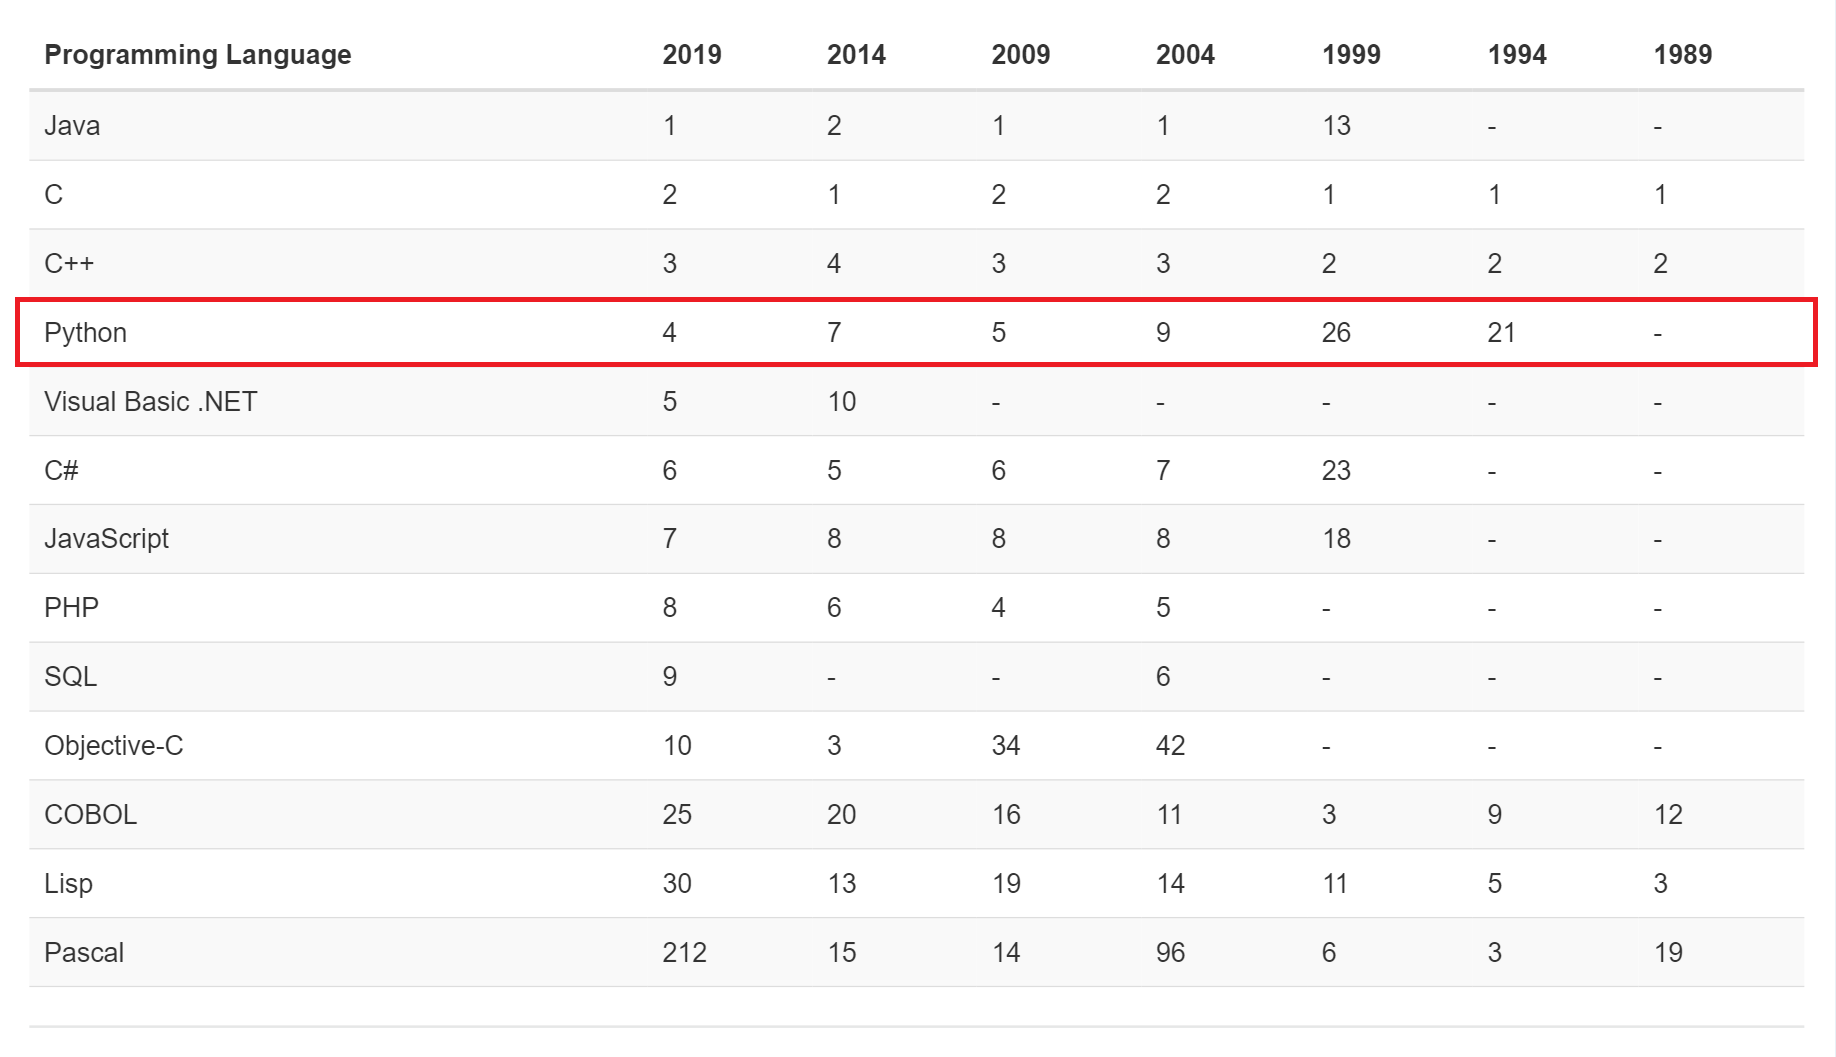
\includegraphics[width=\linewidth]{tiobe.png}
    \caption{Dlouhodobá meziroční statistika oblíbenosti programovacích jazyků podle indexu TIOBE, převzato z \cite{tiobe}}
    \label{fig:tiobe}
\end{figure}

Důvodů k jeho oblibě je hned z několik. Hlavním z nich je srozumitelnost produkovaného kódu a tudíž jeho snadná osvojitelnost i pro uživatele bez větších zkušeností s programováním. S tím souvisí široká uživatelská komunita, která je, vedle propracované dokumentace, důležitým nástrojem při řešení problémů. Jedná se rovněž o multiplatformní jazyk, tj. programy v něm napsané lze bez větších problémů spustit prakticky v libovolném operačním systému, ať už Windows nebo v systémech na bázi Unix (Linux, Mac OS X apod.). V neposlední řadě je značnou výhodou Pythonu jeho rozsáhlá standardní knihovna, která umožňuje celou řadu úkonů. Zároveň je ale pro specializované operace k dispozici velké množství doplňkových knihoven třetích stran.
\vskip 0.1in
\noindent Jak již bylo řečeno, Python je především objektově orientovaným jazykem. Podstatu objektově orientovaného přístupu tvoří tzv. objekty. Objekty jsou seskupení dat s určitými vlastnostmi a funkcionalitami pracující na principu černé skříňky, tj. vykonávají činnosti a komunikaci s okolím bez nutnosti znát jejich vnitřní podstatu. Nadřazeným prvkem objektu je datový typ, neboli třída. Ten sdružuje samotné objekty a také operace, které je možné s nimi provádět. Příkladem může být např. třída \texttt{int} a do ní náležící objekt, číslo \texttt{3}. Třída \texttt{int} tedy pracuje s celými čísly (v počítači ukládána s konečným počtem desetinných míst, z angl.\textit{integers}), s nimiž je možné provádět matematické operace (sčítání, dělení, násobení\ldots), zápis do vektorů a matic apod. \par
Výhoda použití objektově-orientovaného přístupu spočívá v tzv. dědičnosti, díky níž objekty náležící do určité podtřídy odvozené od třídy hlavní přebírají (dědí) její vlastnosti. Tím dochází k úspoře vyprodukovaného kódu, neboť tyto objekty z podtříd není nutné znovu specifikovat. Vzniklý kód je tak přehlednější a celkově úspornější. Toho lze využít např. při tvorbě uživatelských rozhraní, kdy jsou kladeny nároky především na velikost skriptu.

\subsection{Grafické uživatelské rozhraní} \label{sec:GUI}
Grafické uživatelské rozhraní, zkráceně GUI (z angl. \textit{Graphical User Interface}), je nástroj, s jehož pomocí je realizována oboustranná interakce mezi programem a uživatelem. Směrem dovnitř přicházejí vstupy zadané uživatelem, na než následně reagují odpovídající výstupy programu. Vstupy jsou uživatelem vysílány pomocí interaktivních ovládacích prvků, např. ve formě tlačítek, posuvníků, rolovacích seznamů apod. Výstupy programu se pak mohou projevovat rovněž nejrůznější způsoby, ať už jako procesy na pozadí nebo přímo akcemi v rámci grafických oken programu. Vnitřní podstatu fungování GUI si pak lze představit jako jakousi \uv{nekonečnou} smyčku událostí, která je vyvolána spuštěním programu a vytvořením hlavního okna s jeho ovládacími prvky. Ta následně čeká na vstup zvenčí. Pakliže takový vstup nepřichází, setrvává ve vyčkávací pozici. Jakmile jej ale dostane, postupuje dle předepsaného algoritmu až na konec, poté se opět vrátí do vyčkávací pozice. Cyklus se opakuje do té doby, než uživatel vyšle signál k ukončení programu. Princip fungování programu s uživatelským rozhraním je schematicky znázorněn na obr. č. \ref{fig:Gui} (převzato z \cite{Python3Summerfield:2} a upraveno).

\begin{figure}[ht!]
    \centering
    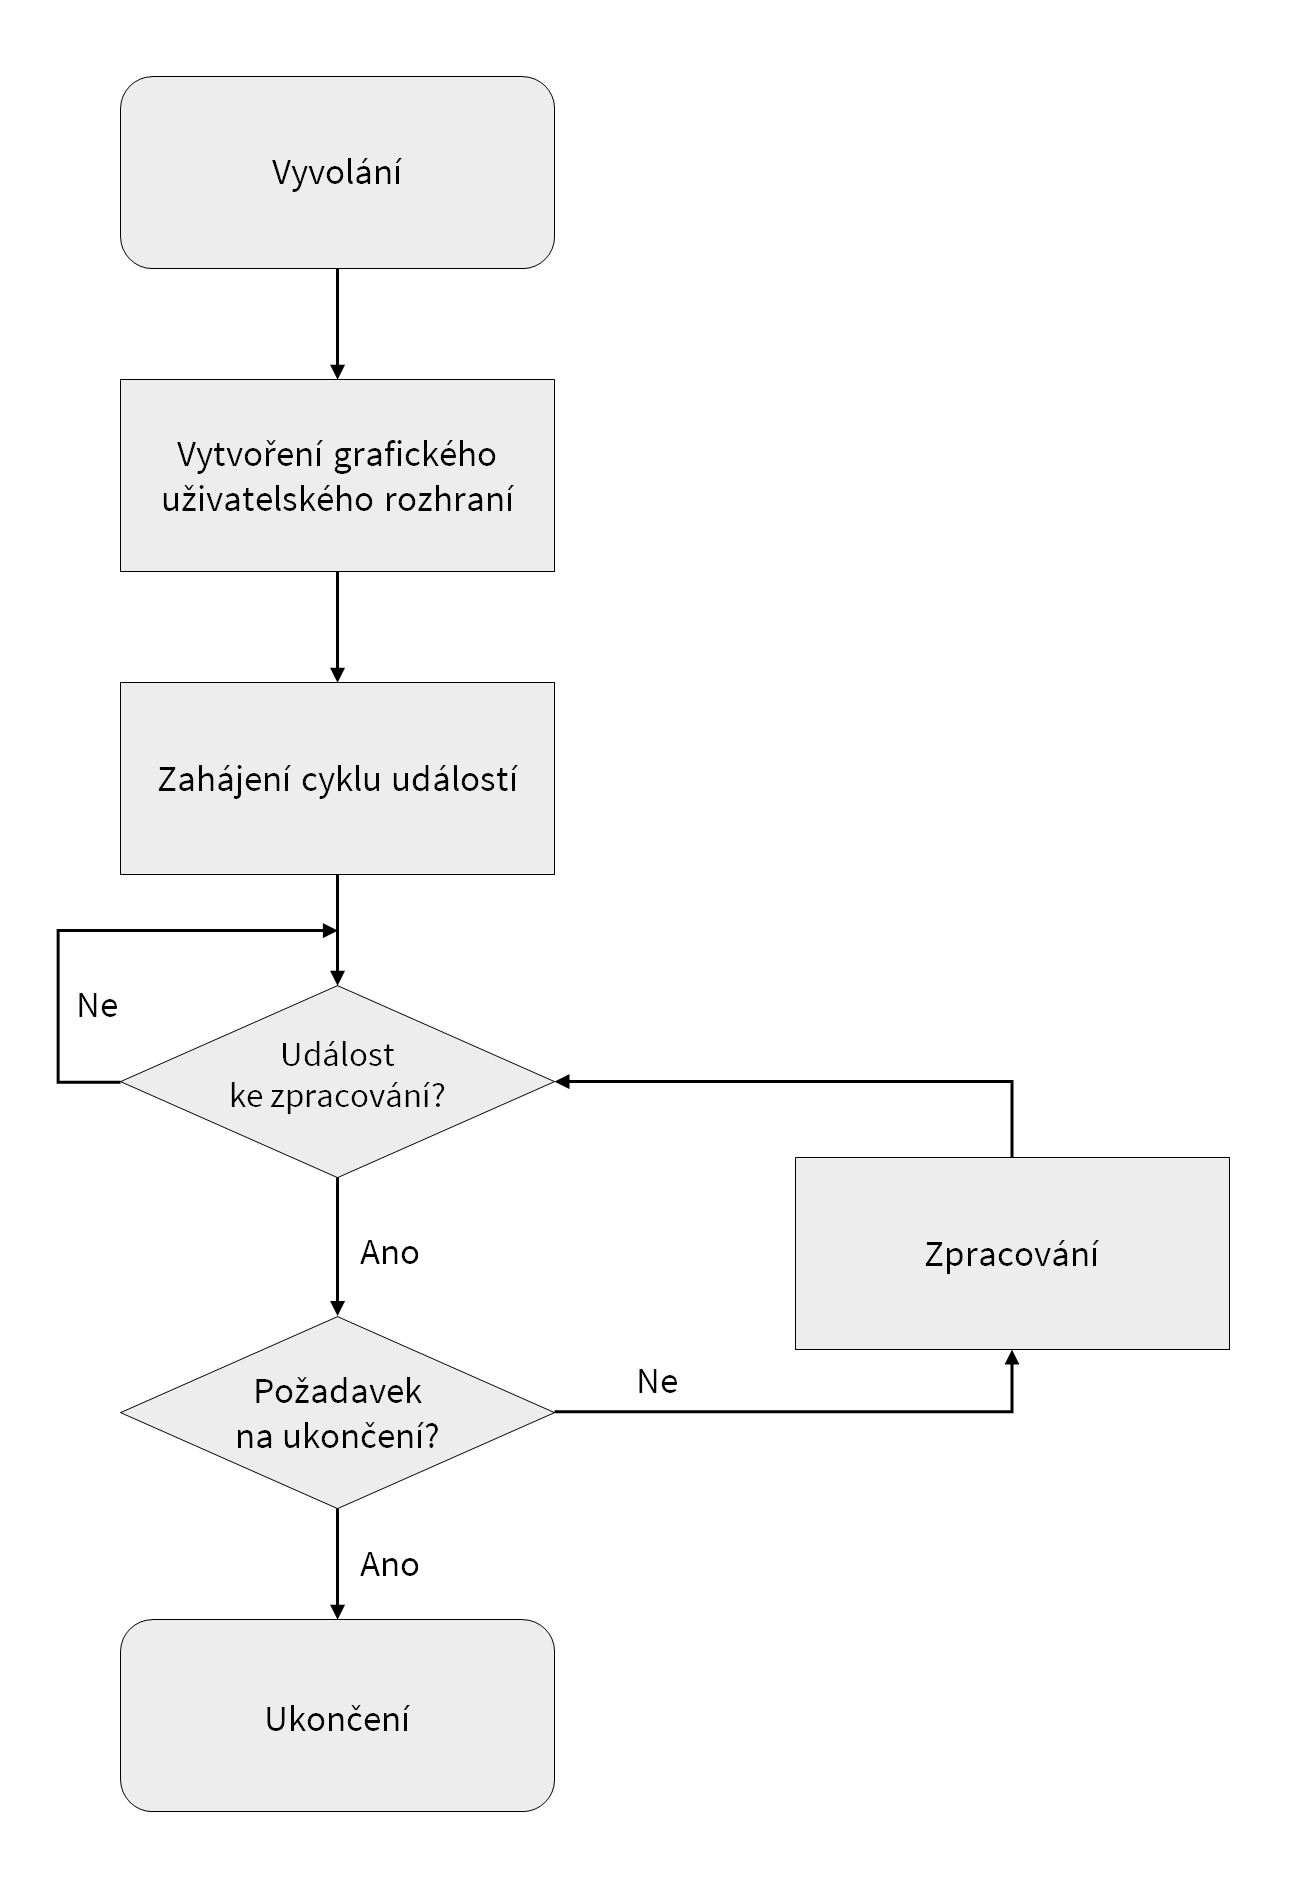
\includegraphics[width=0.8\linewidth,height=14.5cm]{gui_princip.png}\vspace{0.25cm}
    \caption{Princip fungování programu vybaveného grafickým uživatelským rozhraním}
    \label{fig:Gui}
\end{figure}

\subsubsection{Tvorba GUI v Pythonu}
 Realizaci grafického uživatelského rozhraní lze v Pythonu provést hned několika způsoby. K dispozici je celá řada tzv. frameworků, tedy souborů specializovaných balíčků a modulů pro tvorbu GUI. Tato práce se však zaměřuje pouze na dva z nich, a to na PyQt a tkinter, za účelem jejich porovnání. PyQt je framework, v němž byl vytvořen program, jenž je předmětem této práce. tkinter byl zvolen k porovnání z důvodu, že se jedná o obecně nejčastěji používaný modul pro tvorbu uživatelských rozhraní v jazyce Python.
\subsubsection*{tkinter}
Obliba tkinter pramení pravděpodobně z toho, že se jedná o vestavěný modul Pythonu, tj. je součástí jeho standardní instalace spolu s knihovnou GUI Tk. To představuje značnou výhodu zejména v případě, že uživatel má k dispozici pouze standardní instalaci Pythonu a nechce či nemůže instalovat knihovny třetích stran. \cite{Python3Summerfield:2} Zároveň je tkinter frameworkem s poměrně malými nároky na paměť a jednoduchou syntaxí. Je tak vhodný zejména pro začátečníky. S tím se ale také pojí jeho hlavní nevýhoda, kterou je omezená nabídka widgetů, tedy ovládacích prvků (z angl. \textit{widget}), kvůli níž programy v něm vyprodukované nepůsobí nativně. tkinter tak není sám o sobě vhodný k tvorbě složitějších aplikací a je proto žádoucí jej, pokud možno, kombinovat s dalšími knihovnami. Co se týče kvality kódu, tkinter ve srovnání s knihovnami třetích stran opět kulhá. Obecně programy používající k tvorbě GUI jiné knihovny Pythonu než Tk poskytují při stejné nebo kratší délce kódu výrazně lepší výsledky. \cite{Python3Summerfield:2}  

\subsubsection*{PyQt}
PyQt je odnoží multiplatformního frameworku Qt určenou speciálně pro Python. Qt je samo o sobě knihovnou jazyka C++, ale podobně jako pro Python existuje v mnoha modifikacích i pro mnoho dalších skriptovacích jazyků (Ruby - QtRuby, C\texttt{\#}, Pascal, Java, atd.). Výhodou PyQt je přehledná a podrobná dokumentace (společná pro všechny odnože), dále snadná instalace, kterou je možné provádět přímo z příkazového řádku příkazem \texttt{'\textbf{pip} install pyqt5'} a v neposlední řadě také nízké nároky na paměť. Aplikace vytvořené v Qt, resp. PyQt jsou nativní, tj. přizpůsobují svůj vzhled operačnímu systému, na kterém jsou spuštěny. PyQt rovněž nabízí možnost využití nástroje QtDesigner, což je vývojové prostředí umožňující poskládat grafické rozhraní z nabídky jednotlivých ovládacích prvků (viz obr. \ref{fig:QtDesigner}). Z prostředí QtDesigneru je dále možné generovat kód vytvořeného GUI do Pythonu a do něj ručně vepsat funkcionality jednotlivých widgetů. Nevýhodou použití tohoto nástroje je ale množství a značná nepřehlednost generovaného kódu, v němž je řada příkazů generována explicitně a je tudíž nadbytečná. 

\begin{figure}[hbt!]
    \centering
    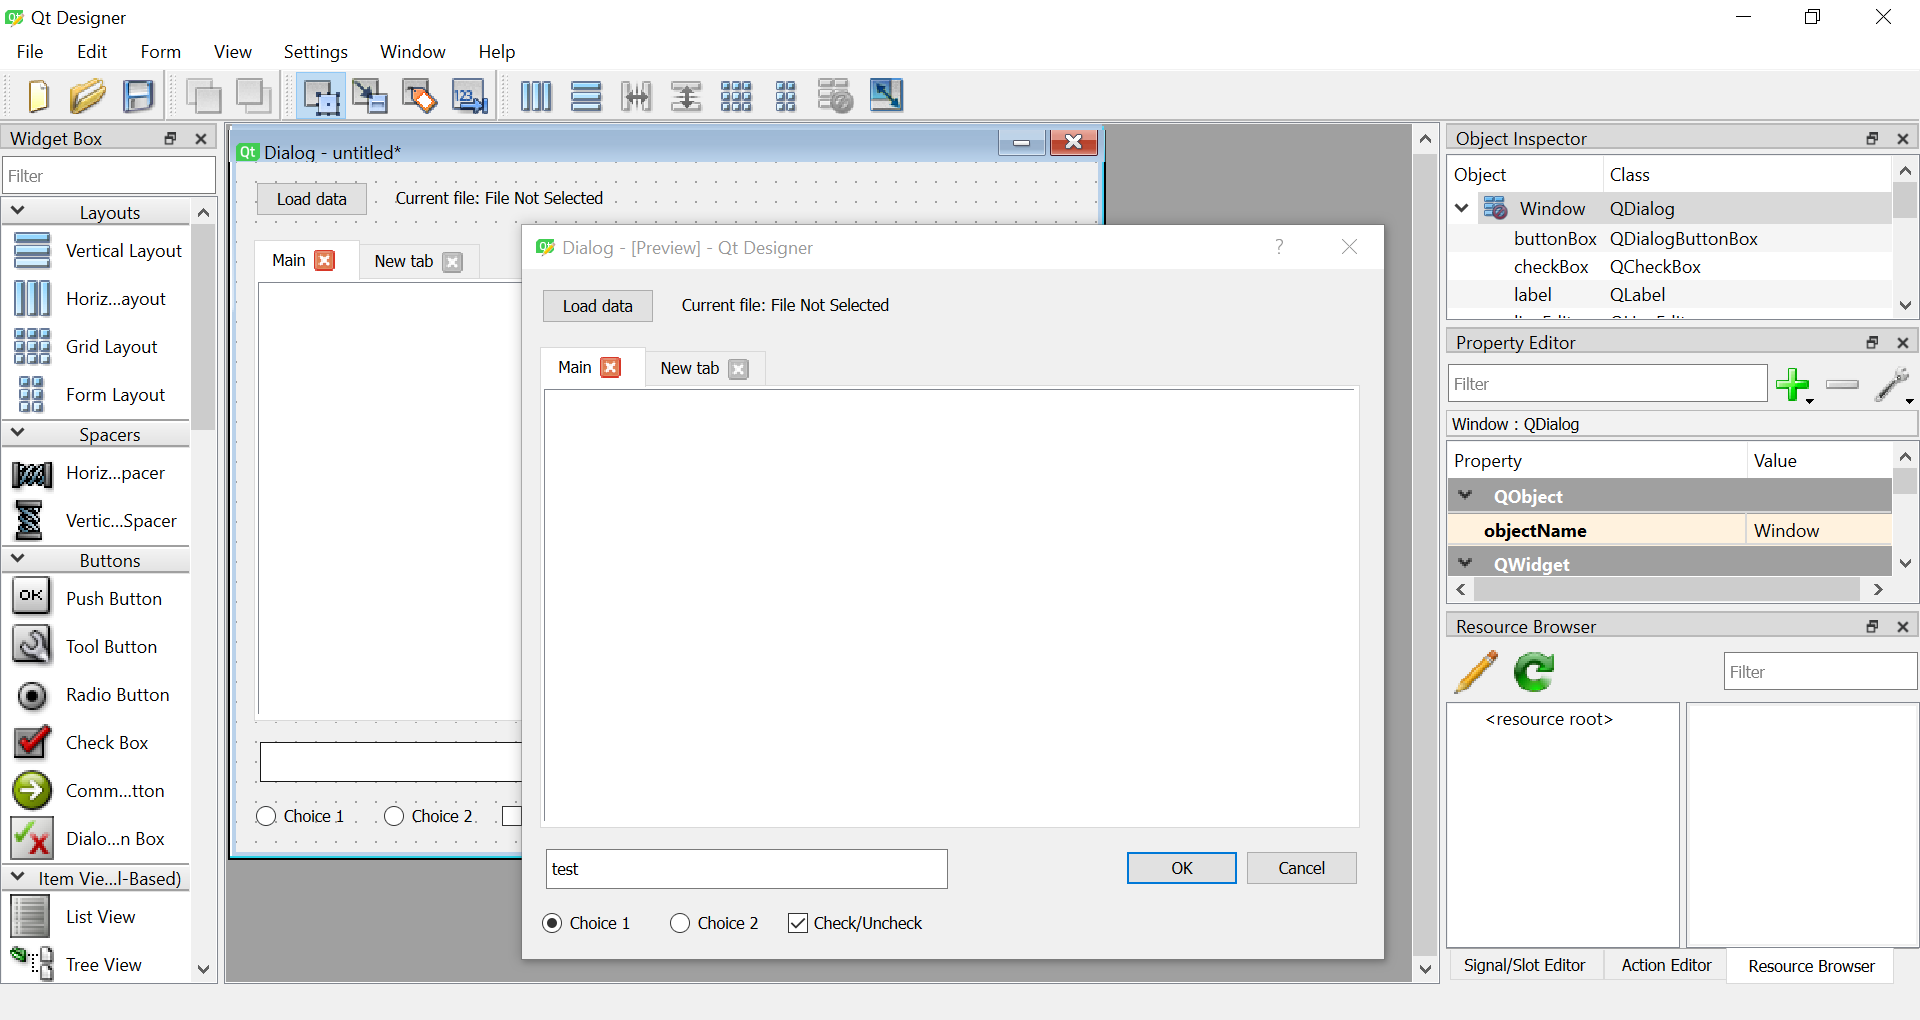
\includegraphics[width=\linewidth,height=9cm]{QtDesigner.png}\vspace{0.4cm}
    \caption{Ukázka použití nástroje QtDesigner}
    \label{fig:QtDesigner}
\end{figure}

\noindent Z pohledu skriptu je proto elegantnějším řešením napsat GUI ručně. Tento přístup je ale na druhou stranu časově výrazně náročnější. Obecně lze říci, že použití QtDesigneru je výhodné při tvorbě jednoduchých aplikací, zejména pro osobní použití, nebo jako podpůrného nástroje pro začátečníky.

Pro komplexnější úlohy se tedy lépe hodí ruční psaní GUI. To sice vyžaduje jistou programovací zkušenost, nicméně nabízí oproti QtDesigneru určitou svobodu v možnosti rozšíření nabídky ovládacích prvků nadefinováním vlastních přímo v kódu a zároveň umožňuje docílit větší přehlednosti a úspornosti skriptu použitím implicitních příkazů.

Pro srovnání obou frameworků byla v každém z nich generována  jednoduchá demonstrační aplikace, jejíž grafické rozhraní sestává z hlavního okna a dvou tlačítek (viz obr. č. \ref{fig:myfirstgui}). Při stisku tlačítka \texttt{Hello world!} program vypíše na konzoli pozdrav \uv{Hello world!}, při stisku druhého tlačítka se program ukončí. Skript obou variant implementace je dostupný v příloze \ref{PrilohaA} této práce.

\begin{figure}[h!]
\centering
\begin{minipage}[b][4cm]{5cm}
  \centering
  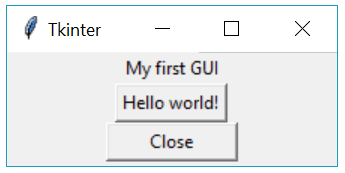
\includegraphics[width=\linewidth]{tkinter_myfirstgui.png}\vspace{0.25cm}
  \subcaption{tkinter}
\end{minipage}\hspace{1.5cm}
\begin{minipage}[b][4cm]{5cm}
  \centering
  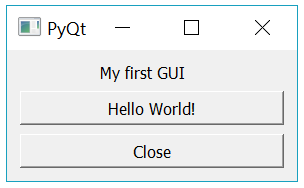
\includegraphics[width=\linewidth]{pyqt_myfirstgui.png}\vspace{0.25cm}
  \subcaption{PyQt}
\end{minipage}\vspace{0.4cm}
\caption{Aplikace \texttt{Hello world!} - ukázka výstupů srovnávaných frameworků}
\label{fig:myfirstgui}
\end{figure}

\newpage
\section{Zpracování signálu} \label{sec:DSP}
Tato kapitola se zaměřuje na vnitřní podstatu programu pro zpracování krystalografických dat, tj. na číslicové zpracování signálu, od stručného nastínění teorie signálů (sekce \ref{sec:signal}), přes problematiku jejich zpracování až ke konkrétním příkladům číslicových filtrů implementovaných v rámci programu (sekce \ref{sec:filtr1} až \ref{sec:filtr4}).
\subsection{Signály} \label{sec:signal}
Signály jsou nositeli informace o podstatě svého zdroje, která je reprezentována okamžitou změnou jedné či více fyzikálních veličin v čase. \cite{uhlíř&sovka2002} Podle povahy signálů je lze dělit např. na spojité a diskrétní. Spojité signály jsou definované pro nekonečně mnoho hodnot nezávisle proměnné veličiny, u diskrétních signálů nezávisle proměnná nabývá pouze hodnot celočíselných. Signály mohou být diskrétní i pro hodnoty závisle proměnné (např. v amplitudě), v takovém případě je nazýváme kvantovanými, popř. číslicovými, jsou-li diskrétní jak v čase, tak v amplitudě (viz obr. č. \ref{fig:signal}).
\begin{figure}[ht!]
\centering
\begin{minipage}[c]{5cm}
  \centering
  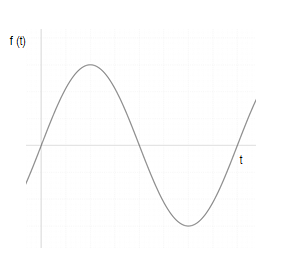
\includegraphics[width=\linewidth]{analogový.png}
  \subcaption{}
\end{minipage}\hspace{1cm}
\begin{minipage}[c]{5cm}
  \centering
  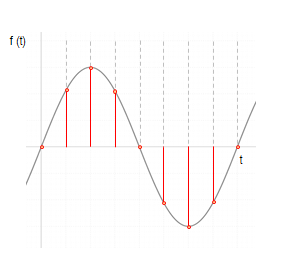
\includegraphics[width=\linewidth]{vzorkovaný.png}
  \subcaption{}
\end{minipage}\vspace{0.25cm}
\begin{minipage}[b]{5cm}
  \centering
  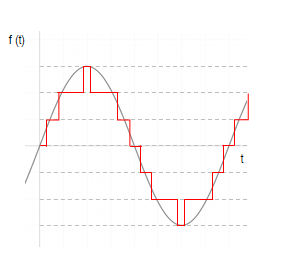
\includegraphics[width=\linewidth]{kvantovaný.png}
   \subcaption{}
\end{minipage}\hspace{1cm}
\begin{minipage}[b]{5cm}
  \centering
  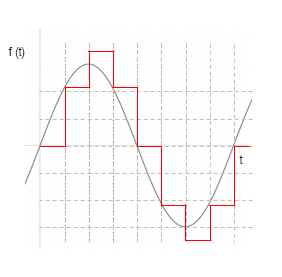
\includegraphics[width=\linewidth]{číslicový.png}
  \subcaption{}
\end{minipage}
\caption{Druhy signálů: a) analogový, b) vzorkovaný, c) kvantovaný, d) číslicový.}
\label{fig:signal}
\end{figure}


Dalším kritériem pro klasifikaci signálů je jejich chování v čase. To je dáno okolnostmi jejich vzniku, fyzikální podstatou a dalšími faktory. V případě, že lze předvídat časový průběh signálu, nazýváme jej signálem deterministickým. V opačném případě, tedy pokud má chování signálu náhodnou povahu, jde o signál stochastický.
Běžné signály jsou obvykle analogového charakteru, tj. spojité v čase i amplitudě. Pro možnost jejich dalšího zpracování je proto potřeba signály při jejich získávání souběžně diskretizovat - sledovaná veličina je snímána pouze v určitých časových okamžicích (vzorkování) a zároveň jsou pomocí vestavěných A/D převodníků kvantovány. Výsledný signál je tak plně digitální, tedy diskrétní v čase i amplitudě. Takto upravený signál je možné podrobit číslicovému zpracování.
Číslicové zpracování se provádí z důvodu potlačení, příp. zvýraznění určitých složek signálu. Složky, které jsou z pohledu sledovaného děje rušivé se nazývají šum a do signálu se dostávají už ve chvíli jeho vzniku, buď z vnitřního prostředí zdroje nebo vlivem okolí. Mezi základní nástroje signálového zpracování patří
analogová a číslicová filtrace, časová, spektrální nebo časově-frekvenční analýza a další.

\noindent Vzhledem ke komplexnosti problematiky zpracování signálu se tato práce zaměří pouze na jeden z jejích nástrojů, a to na číslicovou filtraci.

\subsection{Číslicová filtrace signálu} \label{sec:filtry)}
Filtrace signálu je proces zprostředkovávaný systémem, číslicovým filtrem, při němž dochází ke změně frekvenčního spektra vstupního signálu za účelem zvýraznění, resp. potlačení některých jeho složek. \cite{filtracedef}
Číslicový filtr charakterizují tři základní vlastnosti - impulzní, přenosová a frekvenční charakteristika, které poskytují kompletní představu o chování filtru. Impulzní charakteristika udává chování filtru vyjádřené jeho odezvou na jednotkový puls. Na základě impulzní charakteristiky lze filtry rozdělit na ty s konečnou  impulzní odezvou (nebo-li FIR, z angl. \textit{finite impulse response}), jejichž impulzní odezva má konečný počet nenulových hodnot, a na ty s nekonečnou impulzní odezvou (nebo-li IIR, z angl. \textit{infinite impulse response}), u nichž je počet nenulových hodnot impulzní odezvy nekonečný. Hlavní předností FIR filtrů je jejich stabilita a také poměrně snadný matematický popis, na druhou stranu jejich chování je poměrně vzdálené od chování ideálních filtrů (obr. č. \ref{fig:filtryfrekvs}). IIR filtry jsou v porovnání s FIR filtry efektivnější, tj. pro nižší řád filtru poskytují lepší výsledky, a to především díky svému rekurzivnímu charakteru. Vyšší efektivita IIR filtrů pak souvisí s nižší výpočetní náročností, která je z hlediska implementace nespornou výhodou. Na druhou stranu, na rozdíl od FIR filtrů hrozí u IIR filtrů potíže se stabilitou, která je dána hodnotami koeficientů přenosové funkce. Aby byl daný filtr stabilní, musí být všechny póly jeho přenosové funkce v absolutní hodně menší než 1, tj. musí ležet uvnitř jednotkového kruhu v rovině $z$. \cite{iir}

Přenosovou charakteristiku filtru je možné získat převedením impulzní charakteristiky do frekvenční oblasti pomocí tzv. Z-transformace:
\begin{equation}
H (z) = \frac{b_0 + b_1·z^{-1} + ... + b_n·z^{-n}}{1 + a_1·z^{-1} + ... + a_m·z^{-m}}
\end{equation}
Přenosová funkce udává odezvu filtru na libovolný vstupní signál. Ekvivalentně je možné získat odezvu filtru konvolucí vstupu s jeho impulzní charakteristikou:
\begin{equation}
y [n] = x [n] * h [n] = \sum_{k = -\infty}^{\infty} x[k]·h[n-k]
\end{equation}

\noindent Frekvenční charakteristika filtru je odvozena od impulzní charakteristiky pomocí diskrétní Fourierovy transformace (DTFT, z angl. \textit{discrete time Fourier transform}).

Podle účelu lze filtry rozdělit na základě jejich frekvenční selektivity na dolní propusti (angl. \textit{low-pass}), horní propusti (angl. \textit{high-pass}), pásmové propusti (angl. \textit{band-pass}) a pásmové zádrže (angl. \textit{band-stop}). Jak je patrné z obr. č.\ref{fig:filtryfrekvs}, filtry typu propust konzervují požadované frekvence signálu a ostatní potlačují, naopak filtry typu zádrž požadované frekvence potlačí a zbytek signálu ponechají bez zásahu.

\begin{figure}[hbt!]
\centering
\begin{minipage}[b]{6.5cm}
  \centering
  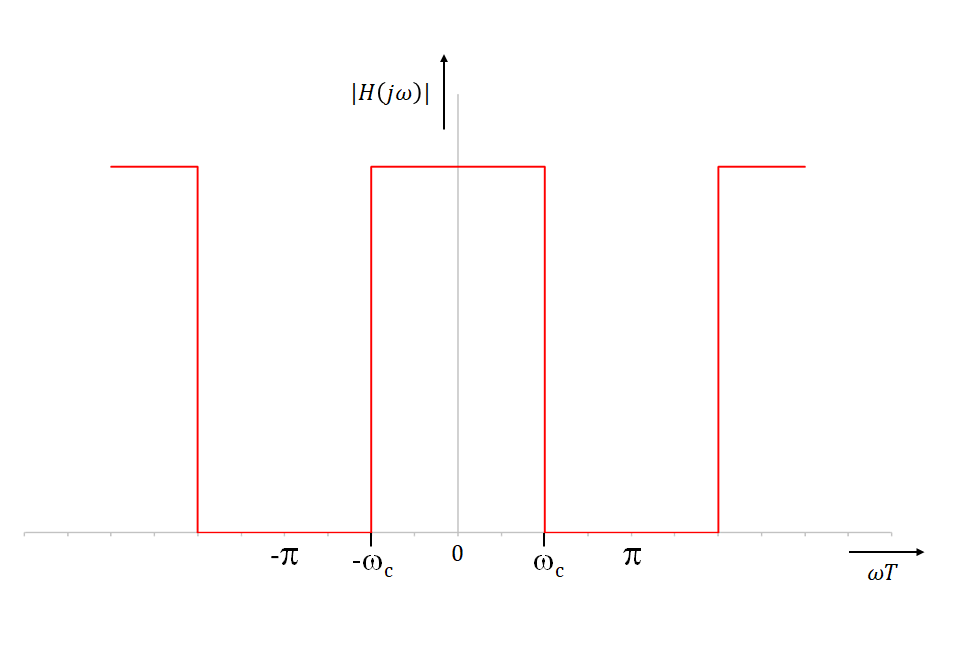
\includegraphics[width=\linewidth]{lowpass.png}\\
  \subcaption{dolní propust}
\end{minipage}\hspace{0.5cm}
\begin{minipage}[b]{6.5cm}
  \centering
  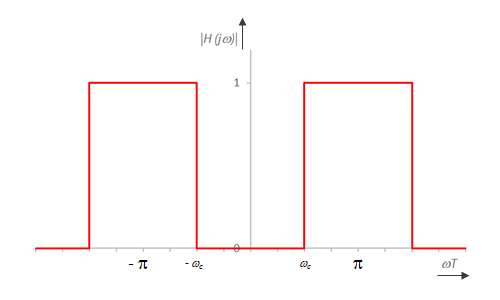
\includegraphics[width=\linewidth]{highpass.png}\\
  \subcaption{horní propust}
\end{minipage}\vspace{0.8cm}
\begin{minipage}[b]{6.5cm}
  \centering
  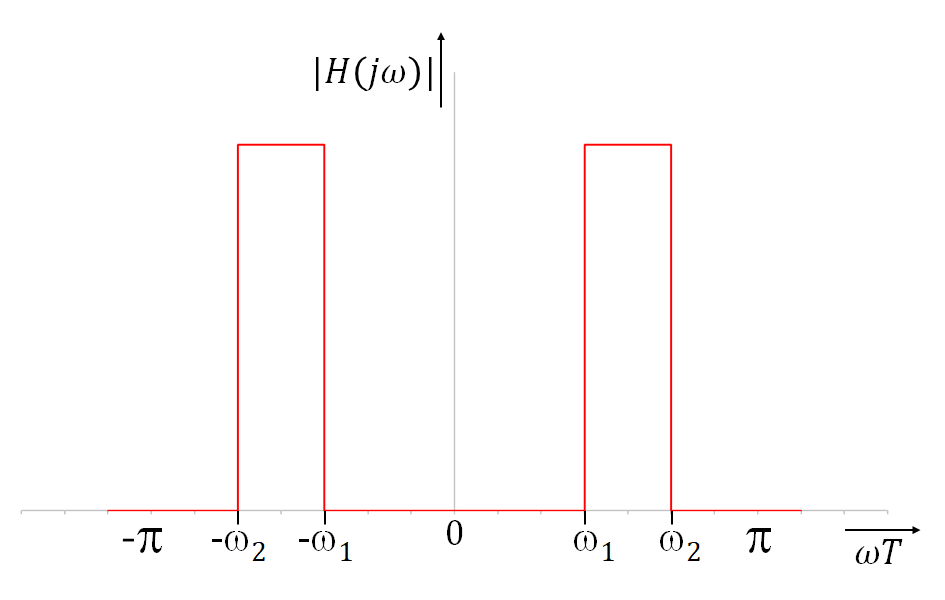
\includegraphics[width=\linewidth]{passband.png}\\
  \subcaption{pásmová propust}
\end{minipage}\hspace{0.5cm}
\begin{minipage}[b]{6.5cm}
  \centering
  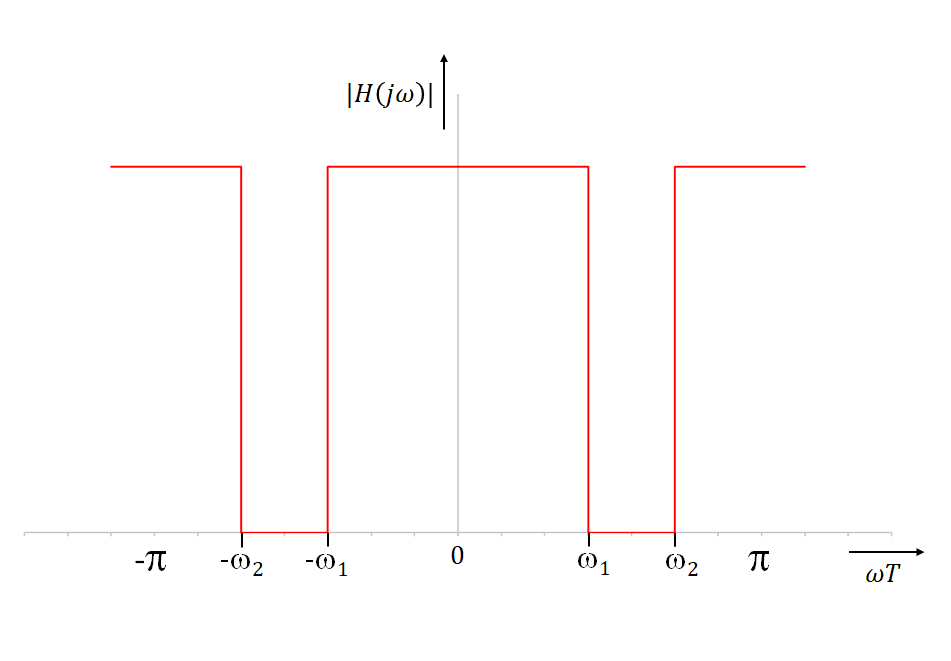
\includegraphics[width=\linewidth]{bandstop.png}\\
  \subcaption{pásmová zádrž}
\end{minipage}\vspace{0.4cm}
\caption{Frekvenční charakteristiky ideálních číslicových filtrů}
\label{fig:filtryfrekvs}
\end{figure}

\textcolor{cdorange}{Chování reálných filtrů se od chování filtrů ideálních liší, a to zejména v rychlosti přechodu do nového ustáleného stavu, který je u reálný filtrů spíše pozvolný než skokový. To, jak moc se filtr blíží svým chováním ideálnímu filtru udává kvalitu jím prováděné filtrace.}

Dále budou blíže popsány konkrétní filtry, které byly zařazeny do programu pro zpracování krystalografických dat. Všechny tyto filtry jsou koncipovány jako low-pass filtry, jsou tedy určeny k eliminaci vysokofrekvenčního šumu.

\subsubsection{Filtr s nulovým fázovým posunem}
\label{sec:filtr1}
Prvním z číslicových filtrů využitých v rámci programu je filtr s nulovým fázovým posunem. K implementaci tohoto druhu filtrace jsou využívány jak filtry FIR typu, tak IIR typu. Ty jsou výpočetně méně náročné, zároveň ale vykazují fázové zkreslení způsobené nelinearitou frekvenční charakteristiky filtru, kdy dochází k nestejnému zpožďování různých složek signálu. U FIR filtrů k tomuto jevu také dochází, zkreslení je však vlivem lineární frekvenční charakteristiky konstantní a nedochází proto k deformaci časové řady. Efekt fázového zkreslení lze částečně potlačit právě zero-phase filtrací. 

Pro docílení nulového fázového posunu se provádí filtrace v dopředném a zpětném směru. To je možné provést dvěma způsoby, buď je nejprve signál filtrován, následně překlopen v čase, poté znova filtrován a nakonec opět překlopen v čase nebo jsou tyto operace provedeny v opačném pořadí, tj. nejprve překlopení signálu v čase a poté filtrace. Oba tyto postupy poskytují ekvivalentní výsledky, jedná se tedy pouze o formální odlišnost ve vnitřním fungování zero-phase systému. Schéma filtrace s nulovým fázovým posunem je znázorněno na obr. č. \ref{fig:zerophase}.
\begin{figure}[hbt!]
  \centering
  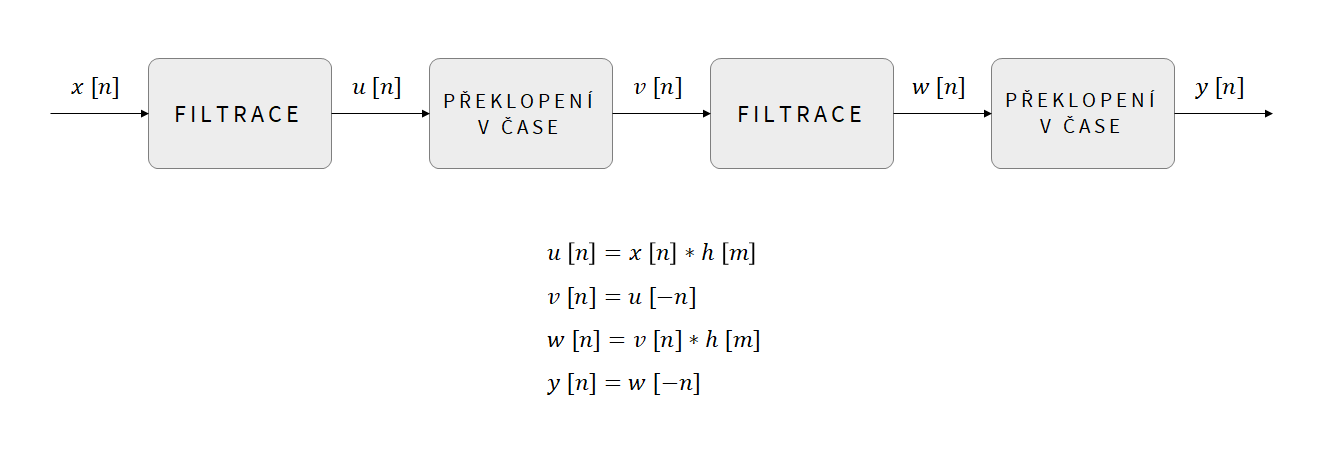
\includegraphics[width=\linewidth]{zero-phase_moje.png}
  \caption{Princip filtrace s nulovým fázovým posunem}
  \label{fig:zerophase}
\end{figure}

\subsubsection{Savitzky-Golay filtr}
\label{sec:filtr2}
\textcolor{cdorange}{Dalším z typů filtrů využitých v rámci programu je Savitzky-Golay filtr (SG filtr).} Jedná se o systém ze skupiny polynomiálních vyhlazovacích filtrů pojmenovaných po analytickém chemikovi Abrahamu Savitzkym a  matematiku Marceli J. E. Golayovi. \cite{SGF} Ti jsou považování za první, kteří navrhli využití tohoto typu systému ke zpracování experimentálních dat. V této oblasti také nalézá svoje největší využití, zejména právě v analytické chemii. Princip Savitzky-Golay filtrů spočívá v proložení podsouboru experimentálních dat polynomem \textit{n}-tého stupně ve smyslu metody nejmenších čtverců a v následném nahrazení \textit{i}-té hodnoty souboru hodnotou daného polynomu. Filtr tedy jinými slovy provádí lokální polynomiální regresi. Vzhledem k symetrii je nutné, aby daný výřez dat (okno) obsahoval lichý počet hodnot.
Filtr lze na signál aplikovat podle rovnice \ref{eq:savgol}.
\begin{equation}
     Y_{j} = \sum_{i=\frac{1-m}{2}}^{\frac{m-1}{2}} C_{i}\ y_{j+i},\qquad \frac{m-1}{2} \leq j \leq n-\frac{m-1}{2}
\label{eq:savgol}
\end{equation}
Hodnoty tzv. konvolučních koeficientů C\textsubscript{i} daného polynomu jsou tabelovány.
Z obr. č. \ref{fig:theo_savitzkygol} je patrné, že při stejné délce okna polynom nižšího stupně více potlačuje zákmity signálu a filtrovaný signál působí hladší, nicméně to může být v určitých druzích aplikací na škodu, neboť právě tzv. píky mohou mít vysokou vypovídací hodnotu o povaze sledovaného děje, která se jejich potlačením znehodnotí.

\begin{figure}[hbt!]
 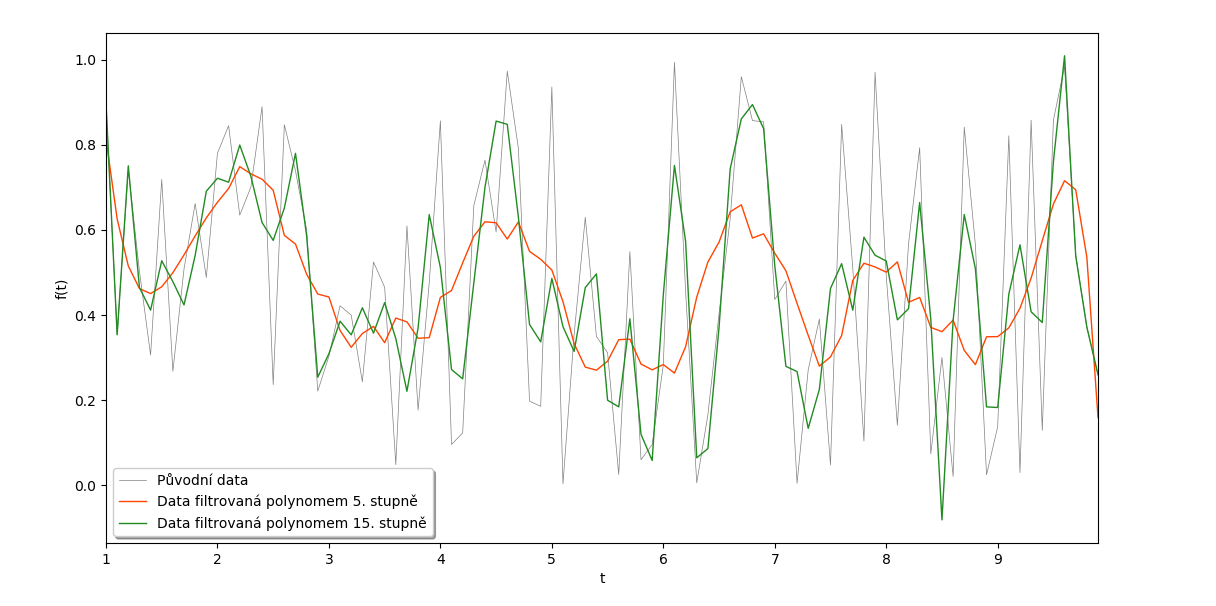
\includegraphics[width=\linewidth]{savgol_.png}
 \caption{Filtrace pseudonáhodného signálu SG filtrem s parametry: stupeň polynomu \textbf{5}, resp. \textbf{15}; velikost okna \textbf{21} hodnot}
 \centering
 \label{fig:theo_savitzkygol}
\end{figure}

textcolor{cdorange}{Použití a návrh SG filtru obecně silně závisí na povaze signálu a zároveň na zkušenostech uživatele, který by měl znát přibližné chování systému, a to v tom smyslu, aby při aplikaci filtru nedošlo k významnému znehodnocení přenášené informace}.
\noindent Filtrace SG filtrem probíhá, na rozdíl např. od klasických FIR/IIR filtrů, v časové oblasti.

\subsubsection{Mediánový filtr}
\label{sec:filtr3}
Dalším z použitých filtrů je filtr mediánový. Principem mediánového filtru je nahradit \textit{i}-tou hodnotu signálu mediánem, tedy prostřední hodnotou, posouvajícího se okna definované délky. Vzhledem k zohledňování předcházejících hodnot při výpočtu odezvy se mediánový filtr řadí mezi nelineární filtry. Pro získání mediánu je potřeba hodnoty v okně nejprve seřadit podle velikosti vzestupně a následně určit prostřední hodnotu podsouboru. Okno může mít libovolný počet hodnot. V případě lichého počtu hodnot v okně je mediánem reálná prostřední hodnota, v případě sudého počtu hodnot je za medián považován aritmetický průměr dvou sousedících prostředních hodnot. Při použití mediánového filtru v některých programovacích jazycích však platí restrikce pouze na okna o lichém počtu hodnot (např. Python - vestavěná funkce knihovny scipy \texttt{medfilt()}). Přes poměrně snadný princip mediánového filtru (viz obr. č. \ref{fig:theo_median}) je při jeho implementaci potřeba ošetřit jeden problém, a to sice výpočet odezvy pro krajní hodnoty datového souboru. K řešení tohoto problému je možné přistoupit dvěma způsoby. V obou případech je nutné chybějící pole pro výpočet mediánu nahradit, a to buď sousedními hodnotami \textit{i}-tého bodu, nebo doplněním chybějících hodnot v okně nulami. Na obrázcích \ref{fig:median_boundary} a \ref{fig:median_zero} jsou uvedeny oba příklady výpočtu odezvy MF na hranici datového souboru pro okno o velikosti 5. Výhody, resp. nevýhody obou přístupů budou rozebrány v diskuzi (sekce \ref{sec:diskuze}) této práce.\vspace{6cm}

\begin{figure}[ht!]
\centering
\begin{minipage}[b]{0.9\linewidth}
  \centering
  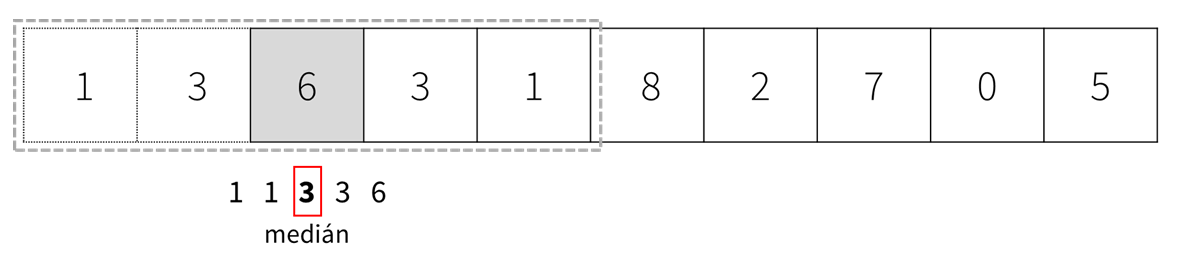
\includegraphics[width=\linewidth]{median_okraj(13).png}\vspace{0.25cm}
  \subcaption{Chování mediánového filtru v krajních bodech datového souboru - nahrazení krajních hodnot sousedními hodnotami}
  \label{fig:median_boundary}
\end{minipage}
\begin{minipage}[b]{0.9\linewidth}
  \centering
  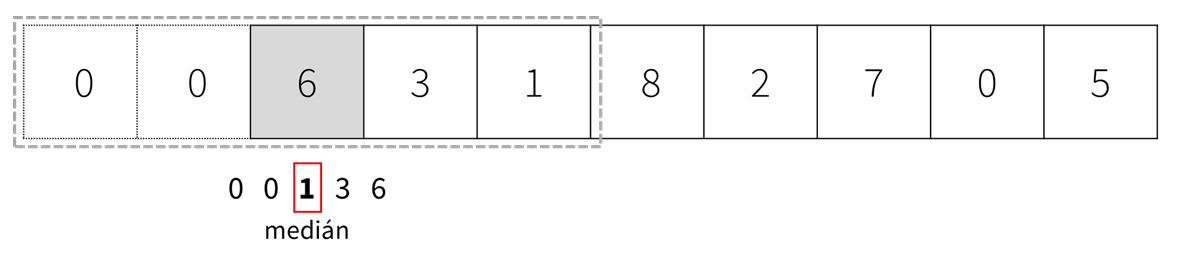
\includegraphics[width=\linewidth]{median_okraj(00).png}\vspace{0.25cm
  \subcaption{Chování mediánového filtru v krajních bodech datového souboru - nahrazení krajních hodnot nulami}
  \label{fig:median_zero}}
\end{minipage}
\begin{minipage}[b]{0.8\linewidth}
  \centering
  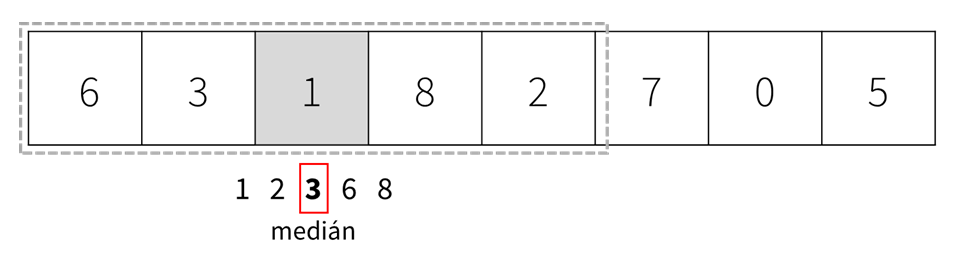
\includegraphics[width=\linewidth]{median_uprostred.png}\vspace{0.25cm
  \subcaption{Chování mediánového filtru uprostřed datového souboru}
  \label{fig:median_middle}}
\end{minipage}\vspace{0.4cm}
\caption{Princip mediánové filtrace}
\label{fig:theo_median}
\end{figure}



\subsubsection{Exponenciální vyhlazování}
\label{sec:filtr4}
Exponenciální vyhlazovací filtr, nebo také exponenciální klouzavý průměr (EMA, z angl. \textit{Exponential Moving Average}), je nástrojem pro analýzu časových řad, díky němuž je možné částečně odhadovat budoucí chování systému v čase. Principem tohoto filtru je váhování předcházejících hodnot ve prospěch hodnot nových, přičemž jako koeficient úměrnosti slouží tzv. vyhlazovací parametr $\alpha$, který nabývá hodnot mezi 0 a 1. Výpočet odezvy filtru lze potom popsat rovnicí \ref{eq:EMA}:
\begin{equation} \label{eq:EMA}
\begin{gathered}
    y_{0} = x_{0}\hspace{6em} \\
    y_{i} = \alpha·x_{i}+(1-\alpha)·y_{i-1},\qquad 0<\alpha<1
\end{gathered}
\vspace{0.25cm}
\end{equation}
Z této rovnice vyplývá, že pro rostoucí hodnotu vyhlazovacího parametru se účinnost filtru snižuje a pro $\alpha$ = 1 je hodnota výstupu rovna hodnotě vstupní. Dosazením vztahu pro výpočet \textit{i}-té výstupní hodnoty do téže rovnice je obdržena geometrická řada objasňující exponenciální podstatu tohoto filtru:
\begin{equation} \label{eq:EMAexp}
    y_{i} = \alpha·[(1-\alpha)·x_{i-1}+(1-\alpha)^{2}·x_{i-2}+_{\ldots}+(1-\alpha)^{i-1}·x_{1}]+(1-\alpha)^{i}·x_{0}
\vspace{0.25cm}
\end{equation}
Závislost váhy hodnoty na její vzdálenosti od současné hodnoty je graficky znázorněna na obr. č. \ref{fig:EMAexp}. Z povahy křivky je patrné, že se skutečně jedná o exponenciálu, navíc s klesající tendencí, z čehož vyplývá, že skutečně čím vzdálenější je hodnota od hodnoty aktuální, tím menší má význam pro výpočet odezvy filtru.


Přidáním dalších vyhlazovacích parametrů lze exponenciální vyhlazování provádět vícenásobně. Dvojité vyhlazování spočívá v zařazení trend vyhlazujícího parametru $\beta$. Trojnásobné vyhlazovaní pak zohledňuje i sezónnost sledovaného děje vnesením třetího parametru $\gamma$. Tyto pokročilé metody ale nejsou předmětem této práce, ta se dále zaměřuje pouze na jednoduché exponenciální vyhlazování.

\begin{figure}[hbt!]
    \centering
    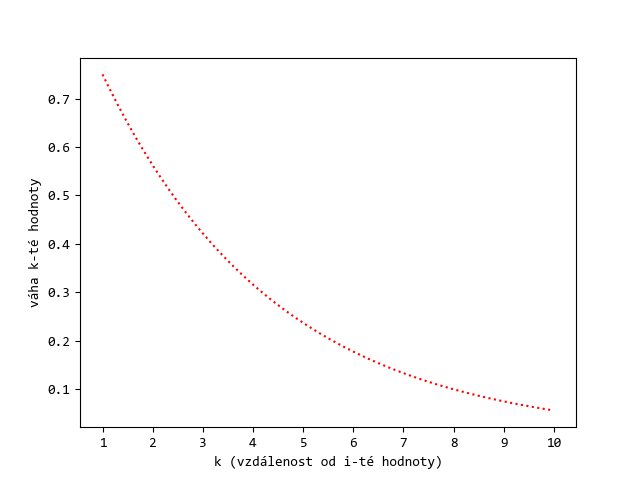
\includegraphics[width=\linewidth,height=8cm]{EMAexp1.png}
    \caption{Křivka závislosti váhy hodnoty (1-$\alpha$) na její vzdálenosti (\textit{k}) od aktuální hodnoty (\textit{$x_i$})}
    \label{fig:EMAexp}
\end{figure}

%%
\clearpage
% praktická část
\section{Tvorba uživatelského rozhraní a zpracování krystalografických dat} \label{sec:prakticka}
Předmětem praktické části této práce byly dva hlavní úkoly, a to implementovat algoritmy pro zpracování dat získaných rentgenovou krystalografií a následně naprogramovat v jazyce Python uživatelské rozhraní umožnující snadnou práci s tímto programem. V následujícím textu bude popsán postup tvorby programu chronologicky tak, jak se předpokládá, že budou jednotlivé prvky využity uživatelem. Tedy od spuštění programu (sekce \ref{sec:mainwin}) až po export zpracovaného signálu do souborů třetích stran (sekce \ref{sec:export}). K tvorbě programu byl použit programovací jazyk Python ve verzi 3.6.6 a některé jeho knihovny, jako např. \textbf{matplotlib}, \textbf{scipy}, \textbf{PySide}, \textbf{numpy} a další. K implementaci uživatelského prostředí pak byla použita knihovna GUI PyQt5 (verze 5.11.3). \textcolor{cdorange}{Zdrojový kód aplikace je přiložen k této práci na CD}.

\subsection{Hlavní okno a funkce} \label{sec:mainwin}
V této kapitole bude rozebrán ústřední funkční prvek aplikace pro zpracování krystalografických dat, hlavní okno a jeho součásti (viz obr. č. \ref{fig:mainWin}).

Před výstavbou samotného GUI je nezbytné vytvořit tělo skriptu obsahující nezbytné náležitosti, jako záhlaví s importem potřebných knihoven a jejich prvků nebo zápatí spouštějící smyčku programu. Dalším krokem je vytvoření hlavního okna a specifikace jeho vlastností. Hlavní okno tvoří tělo celého programu, na nějž jsou navázány další funkce a widgety. V případě programu pro zpracování XRD dat hlavní okno obsahuje widgety pro otevření datového souboru ke zpracování, import dat z něj a nástroje pro vizualizaci. Tyto funkce budou blíže popsány níže.

\subsubsection{Import dat a jejich vizualizace} \label{sec:import}
Proces zpracování krystalografických dat začíná načtením naměřených dat ze souboru. To lze provést stisknutím tlačítka \uv{Open file}, které otevře dialogové okno pro výběr požadovaného souboru. Dialogové okno je realizováno pomocí vestavěné funkce knihovny PyQt5:
\begin{center}
 \texttt{PyQt5.QtWidgets.QFileDialog.getOpenFileName()}.   
\end{center}
\noindent Podporovaným datovým typem je textový soubor s tabulátorovým oddělovačem (.dat). Data jsou ze souboru načtena do matice odpovídající velikosti. Po provedení výběru souboru se dialogové okno automaticky uzavře a zároveň se v horní části okna zobrazí cesta v adresáři k vybranému souboru. V případě opuštění dialogového okna bez výběru souboru program vypíše chybovou hlášku. 

Pro vizualizaci dat slouží centrální widget hlavního okna, do něhož je umístěno plátno knihovny matplotlib. Na ose \textbf{x} je vynesen čas, na ose \textbf{y} úhel ohybu paprsku ($\theta$) a na ose \textbf{z} intenzita prošlého RTG záření. S grafem je možno podle potřeb uživatele otáčet, přibližovat jej atp., a to pomocí ovládacího panelu v dolní části okna.

\begin{figure}[hbt!]
    \centering
    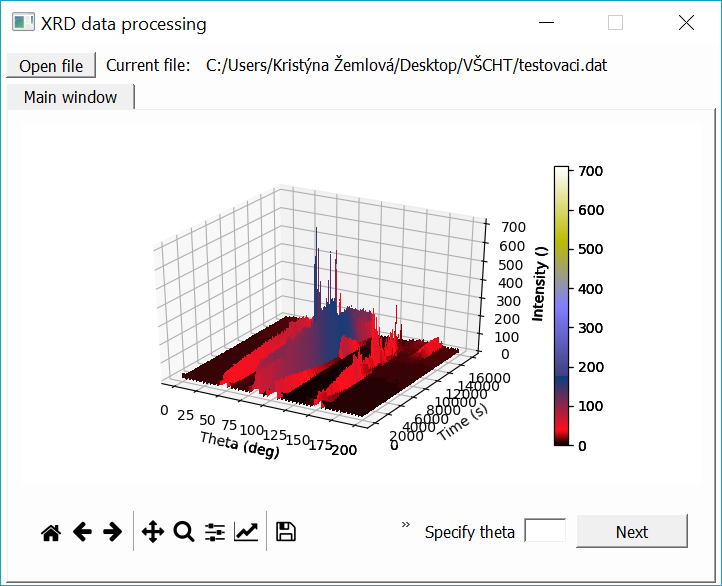
\includegraphics[width=\linewidth]{mainWin_grph.PNG}
    \caption{Hlavní okno programu}
    \label{fig:mainWin}
\end{figure}

\subsubsection{Práce s daty, výběr kanálu} \label{sec:channel}
Po vykreslení dat a jejich vizuálním posouzení je možné v pravé dolní části hlavního okna provést výběr kanálu, tedy výřezu dat pro daný úhel $\theta$, který je z pohledu vyhodnocení zajímavý. Stisknutím tlačítka \uv{Next} dojde k potvrzení výběru a zároveň je vyslán příkaz k otevření nové záložky, kde je možné vzniklý jednorozměrný signál dále zpracovat (viz \ref{sec:fcntabs}). Výběr datového kanálu lze provádět opakovaně zadáním nové hodnoty $\theta$ do editovatelného pole.

\subsection{Záložky a funkce} \label{sec:fcntabs}

Piece of shit:\textcolor{cdorange}{V dalším kroku je vybrané pásmo signálu odpovídající zadanému úhlu $\theta$ vykresleno v nové záložce. Systém okna se záložkami byl zvolen pro větší přehlednost a zároveň umožní zpracování více kanálů najednou. Jednotlivé výřezy je tak možné vzájemně porovnávat jednoduchým přepínáním mezi záložkami. Záložky lze také v rámci lišty libovolně přesouvat potažením myši. Počet otevřených záložek prakticky není omezen, lze jej redukovat uzavřením dané záložky pomocí křížku. Záložku hlavního okna s dvourozměrnou grafikou zavřít nelze.}
\vskip 0.3in
\ldots
\vskip 0.3in
\begin{figure}[hbt!]
    \centering
    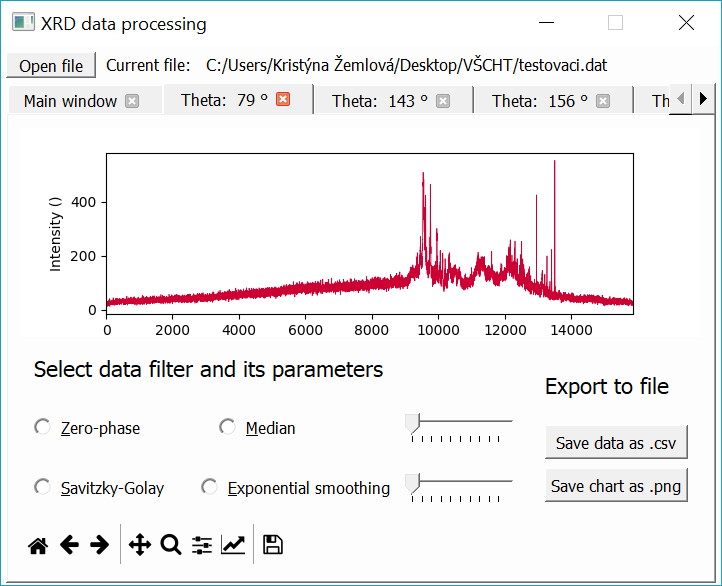
\includegraphics[width=\linewidth]{gui_tab.png}
    \caption{Hlavní okno se záložkami}
    \label{fig:gui_tab}
\end{figure}

\subsubsection{Filtrace signálu}\label{sec:exp_filtrace}
Zpracování signálu je v rámci programu prováděno číslicovou filtrací. Výběr požadovaného filtru se provede v sekci filtrace stiskem příslušného zaškrtávacího tlačítka označeného názvem filtru.

\noindent Do programu byly zařazeny celkem čtyři různé číslicové filtry (viz obr. č. \ref{fig:exp_filtry}), z nichž dva byly realizovány pomocí vestavěných funkcí knihovny \textbf{scipy} a dva byly implementovány. Princip jejich fungování je blíže popsán v kapitolách \ref{sec:filtr1} až \ref{sec:filtr4} této práce.
\vskip 0.1in
\noindent Prvním z použitých filtrů je tzv. zero-phase filtr, k jehož realizaci byla využita funkce knihovny \textbf{scipy} \texttt{signal.filtfilt()}. Parametry této funkce představují koeficienty přenosové funkce FIR filtru $b$, resp. $a$ a posloupnost filtrovaného signálu. Parametry $a$ a $b$ byly optimalizovány na základě vizuálního posouzení filtrovaného signálu a v rámci programu je nelze uživatelem měnit.

Obdobný přístup byl zvolen i u druhého z použitých filtrů, Savitzky-Golay filtru, jehož parametry byly rovněž optimalizovány a jsou v programu pevně nastaveny. Pro realizaci SG filtru byla použita vestavěná funce knihovny \textbf{scipy} \texttt{signal.savgol}\verb|_|\texttt{filter()}, jejímiž parametry jsou velikost okna filtrovaného signálu a stupeň regresního polynomu.

Třetím zařazeným filtrem je filtr mediánový, který byl v rámci programu implementován. K implementaci MF byl použit \textbf{\texttt{\textcolor{royalblue(traditional)}{for}}} cyklus a výpočet odezvy v krajních bodech byl ošetřen větvením. Chybějící hodnoty okna jsou nahrazovány sousedními hodnotami \textit{i}-tého bodu. Výpočet samotného mediánu je pak prováděn pomocí vestavěné funkce knihovny \textbf{numpy} \texttt{np.median()}. Velikost okna filtru je možné regulovat prostřednictvím posuvníku náležícího danému filtru. 
\vskip 0.2in
\begin{lstlisting}[language=Python,numbers=none,frame=single]
# s ... cas
# r ... posloupnost vstupniho signalu

mf = np.zeros(len(s))
for i in range(len(s)):
    k = (win - 1) // 2
    q = r[i + 1:((i + 1) + k)]
    n = r[(i - k):i]
    u = r[i + 1:i + (k - i) + 1]
    # levy okraj datoveho souboru
    if i < k:
        a = np.concatenate((u[::-1], r[:i + 1], q), axis=None)
        mf[i] = np.median(a)
    # pravy okraj datoveho souboru
    elif (i + ((win - 1) // 2)) > (len(s) - 1):
        p = r[i - k:i - (len(s) - 1 - i)]
        b = np.concatenate((n, r[i:], p[::-1]), axis=None)
        mf[i] = np.median(b)
    # stred datoveho souboru
    else:
        c = r[i - ((win - 1) // 2):(i + ((win + 1) // 2))]
        mf[i] = np.median(c)
\end{lstlisting}
\vskip 0.2in
Implementován byl i poslední z filtrů, exponenciální vyhlazovací filtr (EMA), a to dle definice (rovnice \ref{eq:EMA}). Parametrem EMA je vyhlazovací parametr $\alpha$, který lze, podobně jako u MF, nastavit uživatelem pomocí posuvníku. \par
Vzhledem k faktu, že parametr $\alpha$ nabývá hodnot mezi 0 a 1, a zároveň s rostoucí hodnotou $\alpha$ klesá míra vyhlazování, bylo potřeba upravit nastavení posuvníku. A to tak, aby hodnota nastavená na posuvníku zcela vlevo odpovídala nejnižší míře vyhlazení a naopak hodnota zcela vpravo nejvyšší míře vyhlazení. Hodnoty nastavené na posuvníku tak oproti výchozímu nastavení klesají zleva doprava. Z pohledu uživatele je však toto nastavení logičtější.

\vskip 0.2in
\begin{lstlisting}[language=Python,numbers=none,frame=single]
# r ... posloupnost vstupniho signalu
# alpha ... vyhlazovaci parametr
# aux ... vystupni posloupnost

aux = np.zeros(r.shape)

for idx, a in np.ndenumerate(r):
    if idx[0] == 0:
        aux[idx[0]] = a  # pocatecni podminka
    else:
        aux[idx[0]] = alpha * a + (1 - alpha) * aux[idx[0] - 1]
\end{lstlisting}
\vskip 0.2in

\subsubsection{Export dat} \label{sec:export}
Poslední fází zpracování krystalografických dat je uložení těchto dat do souboru přístupného i po opuštění programu. Program nabízí dvě možnosti exportu zpracovaných dat, a to buď ve formě prostého textu nebo ve formě grafiky.
Stisknutím tlačítka pro uložení (\uv{Export data} - viz obr. č. \ref{fig:gui_tab}) se otevře systémové dialogové okno realizované vestavěnou funkcí knihovny PyQt5:
\begin{center}
 \texttt{PyQt5.QtWidgets.QFileDialog.getSaveFileName()},   
\end{center}
jejímž výstupem je vybraná cesta v adresáři a zadaný název novému souboru. Cesta slouží jako vstupní argument další vestavěné funkce, \texttt{np.savetxt()} knihovny \textbf{numpy}, která data uloží do textového souboru s čárkovým oddělovačem. S takto uloženými daty je možné dále pracovat např. v tabulkovém procesoru MS Excel.

Při ukládání grafické podoby zpracovaných dat se, obdobně jako v předcházejícím případě, po stisku tlačítka \uv{Save chart} otevře systémové dialogové okno. V tomto případě je kromě zadané cesty v adresáři argumentem ukládající funkce i požadovaná koncovka nového souboru. Podporovanými datovými typy jsou *.png (\textit{Portable Network Graphics}), *.jpg nebo *.svg (\textit{Scalable Vector Graphics}). Obdobnou funkci jako tlačítko \uv{Save chart} má ikona \hspace{0.09cm}\Icon\hspace{0.09cm} na panelu nástrojů v dolní části okna, která však umožňuje ukládat grafy pouze ve formátu *.png.

\newpage

\section{Výsledky a diskuse} \label{sec:diskuze}
V první fázi tvorby programu byla řešena otázka volby knihovny GUI, ve které bude rozhraní programu implementováno. Vzhledem ke komplexnosti úlohy byla nakonec vybrána knihovna GUI PyQt5, která oproti standardní knihovně Tk nabízí širší možnosti dalšího rozvoje programu \ldots
\vskip 0.5in

Testování chodu programu bylo prováděno na souboru testovacích dat\footnote{Soubor \uv{\texttt{testovaci.dat}} je spolu se zdrojovým kódem programu přiložen k této práci na CD.} o rozměrech 15853 řádků a 207 sloupců (odpovídá velikosti 34.4 MB)

\vskip 0.5in
\begin{figure}[hbt!]
 \centering
 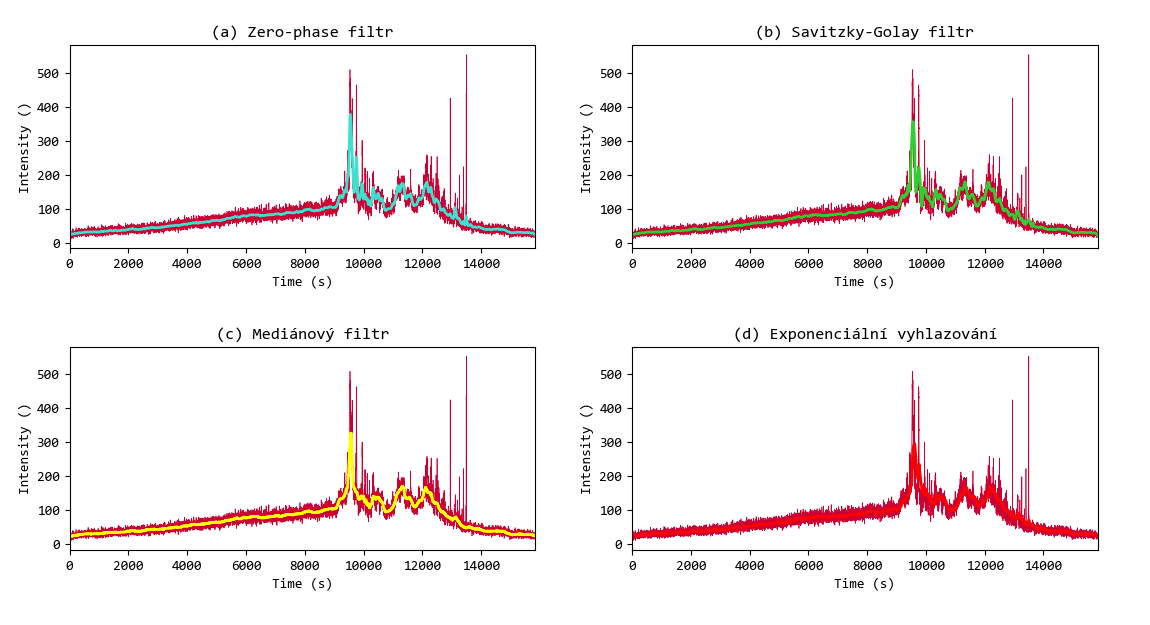
\includegraphics[width=\linewidth,height=0.65\linewidth]{exp_figures.png}
 \caption{Ukázka výstupů filtrace v rámci programu: kanál \textbf{79}}
 \label{fig:exp_filtry}
\end{figure}


\newpage
\section{Závěr}


% seznam literatury
\newpage

\bibliography{citace}
%%

% seznam obrázků
\newpage
\listoffigures
%%

% přílohy
\newpage
\section*{Přílohy}
\addcontentsline{toc}{section}{Přílohy}
\appendix
\section{Zdrojové kódy miniaplikace \texttt{Hello world!}}
\label{PrilohaA}
\subsection{Miniaplikace \texttt{Hello world!} vytvořená v tkinter}
\begin{lstlisting}[language=Python]
from tkinter import Tk, Label, Button

class MyFirstGUI:
    def __init__(self, window):
        self.window = window
        window.title("Tkinter")
        self.label = Label(window, text="My first GUI")
        self.label.pack()
        self.hello_button = Button(window, text="Hello world!", command=self.sayhello)
        self.hello_button.pack()
        self.close_button = Button(window, text="       Close      ", command=window.quit)
        self.close_button.pack()

    def sayhello(self):
        print("Hello world!")

root = Tk()
my_gui = MyFirstGUI(root)
root.mainloop()
\end{lstlisting}
\newpage
\subsection{Miniaplikace \texttt{Hello world!} vytvořená v PyQt5}
\begin{lstlisting}[language=Python]
import sys
from PyQt5 import QtCore, QtWidgets
from PyQt5.QtWidgets import QMainWindow, QLabel, QPushButton, QGridLayout, QWidget
from PyQt5.QtCore import QSize

class HelloWindow(QMainWindow):
    def __init__(self):
        QMainWindow.__init__(self)
        self.setMinimumSize(QSize(300, 60))
        self.setWindowTitle("PyQt")
        centralWidget = QWidget(self)
        self.setCentralWidget(centralWidget)

        gridLayout = QGridLayout(self)
        centralWidget.setLayout(gridLayout)

        hello = QPushButton("Hello World!", self)
        hello.clicked.connect(self.hellofcn)
        close = QPushButton("Close", self)
        close.clicked.connect(self.close)
        label = QLabel("My first GUI")
        label.setIndent(100)

        gridLayout.addWidget(label, 0, 0)
        gridLayout.addWidget(hello, 1, 0)
        gridLayout.addWidget(close, 2, 0)

    def hellofcn(self):
        print("Hello world!")


if __name__ == "__main__":
    app = QtWidgets.QApplication(sys.argv)
    mainWin = HelloWindow()
    mainWin.show()
    sys.exit( app.exec_() )
\end{lstlisting}
%

\end{document}
